% Created 2015-10-27 ti 21:28
\documentclass[12pt,a4paper,english]{tutthesis}
% Note that you must choose either Finnish or English here and there in this
% file.
% Other options for document class
  % ,twoside,openright   % If printing on both sides (>80 pages)
  % ,twocolumn           % Can be used in lab reports, not in theses

% Ensure the correct Pdf size (not needed in all environments)
\special{papersize=210mm,297mm}


% LaTeX file for BSC/MSc theses and lab reports.
% Requires the class file (=template) tutthesis.cls, tut-logo,
% exampleFig (as pdf or eps) and example_code.c
% Author: Sami Paavilainen (2006)
% Modified: Heikki Huttunen (@tut.fi) 2012-07-31
%           Erno Salminen   (@tut.fi) 2014-08-15
%             - added text snippets from the writing guide
%             - added lots of comments: both tips and alternative styles
%             - added an example table
%             - and so on...

%
% Define your basic information
%
\author{Riku Itäpuro}
\title{Thesis title}      % primary title (for front page)
\titleB{Otsikko suomeksi} % translated title for abstract
\thesistype{Master of Science thesis} % or Bachelor of Science, Laboratory Report... 
\examiner{Vilma Valkky} % without title Prof., Dr., MSc or such

% Special trick to use internal macros outside the cls file
% (e.g. @author). Trick is reversed with makeatother a bit later.
\makeatletter

% Define the pdf document properties
\hypersetup{   
  pdftitle={\@title},
  pdfauthor={\@author},
  pdfkeywords={transmogrifier design analysis}
}
\usepackage[finnish, english]{babel}


\author{Riku Itäpuro}
\title{Smartphone as a trust anchor for delegated home net configuration management}
\titleB{Älypuhelin kotiverkkojen luottamusankkurina}
% Ensure the correct Pdf size (not needed in all #+LATEX_HEADER: \special{papersize=210mm,297mm}
\thesistype{draft-27.10.2015 Master of Science thesis}
\examiner{Jarmo Harju}
\makeatletter
\usepackage{svg}
\usepackage[utf8]{inputenc}
\usepackage[all]{nowidow}
\author{Riku Itäpuro}
\date{27.10.2015 \{12., 8, 3.10., 28.,2.9., 20.,18.8.,27.7,11.5,7.5.to the github,28.4, 16.4, 13.4.2015 new-framing, 4.4, 27.3,  20.3, 7.3)}
\title{Smartphone as a trust anchor in home networks}
\hypersetup{
  pdfkeywords={},
  pdfsubject={},
  pdfcreator={Emacs 24.4.1 (Org mode 8.2.10)}}
\begin{document}

\maketitle



 \hypersetup{  
 pdfkeywords={authentication, authorization, AAA, homenet, smartphone, trust anchor, EAP-SIM, RADIUS}
}
\chapter*{Terminology}
%\chapter*{Lyhenteet ja merkinn<E4>t}
\markboth{}{}                                % no headers

If not already on vocabulary, expansion of the most important terms like
authentication, key-exchange, integrity, replay, algorithms, SIM,\ldots{}

\newpage             % Added 2015-02-22

 \pagenumbering{Roman}
 \pagestyle{headings}
% \begin{document}
%  title page 
 \thispagestyle{empty}
\date\today
 \vspace*{-.5cm}\noindent
 
\includegraphics[width=8cm]{tty_tut_logo}   % Bilingual logo

% lay out author, title and type 
\vspace{6.8cm}
\maketitle
%\vspace{7.7cm} % -> 6.7cm if thesis title needs two lines
\vspace{6.7cm} % -> 6.7cm if thesis title needs two lines

% Last some additional info to the bottom-right corner
\begin{flushright}  
  \begin{minipage}[c]{6.8cm}
    \begin{spacing}{1.0}
      %\textsf{Tarkastaja: Prof. \@examiner}\\
      %\textsf{Tarkastaja ja aihe hyväksytty}\\ 
      %\textsf{xxxxxxx tiedekuntaneuvoston}\\
      %\textsf{kokouksessa 4.2.2015}\\
      \textsf{Examiner: Prof. \@examiner}\\
      \textsf{Examiner and topic approved by the}\\ 
      \textsf{Faculty Council of the Faculty of} \\
      \textsf{Computing and Electrical Engineering} \\
      \textsf{on 4th February 2015}\\
    \end{spacing}
  \end{minipage}
\end{flushright}


% Leave the backside of title page empty in twoside mode
\if@twoside
\clearpage
\fi


\pagenumbering{roman}
\setcounter{page}{0} % Start numbering from zero because command 'chapter*' does page break

%%% \begin{otherlanguage}{english} %  Following text in in 2nd language
\chapter*{Abstract}

\begin{spacing}{1.0}
  {\bf \textsf{\MakeUppercase{\@author}}}: \@title\\   % use \@titleB when thesis is in Finnish
   \textsf{Tampere University of Technology}\\
   \textsf{\@thesistype, xx pages, x Appendix pages} \\
   \textsf{xxxxxx 2015}\\
   \textsf{Master's Degree Programme in Information Technology}\\
   \textsf{Major: Information Security}\\
   \textsf{Examiner: Prof. \@examiner}\\ % 
   \textsf{Keywords: authentication, authorization, AAA, homenet, smartphone, SIM, trust-anchor, EAP-SIM, RADIUS}\\
\end{spacing}

%---------------------------------------------------------
%   A B S T R A C T
% [The abstract is a concise 1-page descriptionof the work: 
[what was the problem, what was done, and what are the results. ]
% Do not include charts or tables in the abstract.

Today, home networks have become more complex and the home owner 
does not necessarily want to administer all aspects of it.
Configuring home network devices does not differ much from configuring enterprise devices. One needs access, credentials to login and knowledge to operate the device. If the configuration is out-sourced to external parties and 
done remotely, those requirements need adjustment.
Access to an end device must be provided from outside. 
A trustful operator must be hired and login credentials shared to them to make configuration changes.
For that,  some beforehand set provisioning and distribution of authentication keys is needed.
As there already exists an infrastructure within mobile phone subscribers, that is used in the study as a trusted base.
To benefit from the mobile identification, it is shown how
the authentication is done using an extendable authentication profile (EAP) with a SIM-card
and how the authorization is checked with a RADIUS protocol.
A theory, how SIM-authentication works is presented and a simulated environment
to demonstrate that is built, tested and analyzed.
As results, it is shown, that SIM authentication's benefits are strong
authentication and existing user-base, while its disadvantages include
dependency to mobile operator. Additionally, there will remain challenges in keeping SIM's identity private and in disabling unwanted re-authentications. % [or: balancing the re-authentication]
The principle has been to reuse existing techniques when combining them to such new areas as homenet and delegated management.
 For transporting authentication claims, WPA2 Enterprise, which includes RADIUS environment has been chosen.
To further avoid complexity and granularity, we
only use a simple model of management network. Getting in to management network is carried out at home network via EAP-SIM authentication and it is the key element of the thesis.



%%%\end{otherlanguage} % End on 2nd language part
%---------------------------------------------------------
%   T I I V I S T E L M Ä 

\begin{otherlanguage}{finnish} %  Following text in in 2nd language
\chapter*{Tiivistelmä}         % Asterisk * turns numbering off

\begin{spacing}{1.0}
         {\bf \textsf{\MakeUppercase{\@author}}}: \@titleB\\  % or use \@title when thesis is in Finnish
         \textsf{Tampereen teknillinen yliopisto}\\
         \textsf{Diplomityö, xx sivua, x liitesivua}\\ %
         \textsf{toukokuu 2015}\\
         \textsf{Tietotekniikan koulutusohjelma}\\
         \textsf{Pääaine: tietoturva}\\
         \textsf{Tarkastaja:  Prof. \@examiner}\\ % automated, if just 1 examiner
         \textsf{Avainsanat: tunnistaminen, valtuutus, AAA, kotiverkko, älypuhelin, luottamusankkuri, EAP-SIM, RADIUS}\\
\end{spacing}
The abstract in Finnish. Foreign students do not need this page.
TBD

Kirjoita, kun english versio on hyvä(ksytty).
\end{otherlanguage} % End on 2nd language part

% varmuuden vuoksi, sillä esim. captioneissa Kuva tulee muuten suomeksi 
%%% \begin{otherlanguage}{english} %  Following text in in 2nd language
\begin{otherlanguage}{english} %  Following text in in 2nd language
\makeatother % Make the @ a special symbol again, as \@author and \@title are not neded after this

%
% PREFACE
%
\chapter*{Preface}

PREFACE TEMPLATE! SKIP.

This document template conforms to Guide to Writing a Thesis at
Tampere University of Technology (2014) and is based on the previous
template. The main purpose is to show how the theses are formatted
using LaTeX (or \LaTeX ~ to be extra fancy) .


The thesis text is written into file \texttt{d\_tyo.tex}, whereas
\texttt{tutthesis.cls} contains the formatting instructions. Both
files include lots of comments (start with \%) that should help in
using LaTeX. TUT specific formatting is done by additional settings on
top of the original \texttt{report.cls} class file. This example needs
few additional files: TUT logo, example figure, example code, as well
as example bibliography and its formatting (\texttt{.bst}) An example
makefile is provided for those preferring command line. You are
encouraged to comment your work and to keep the length of lines
moderate, e.g. <80 characters. In Emacs, you can use \texttt{Alt-Q} to
break long lines in a paragraph and \texttt{Tab} to indent commands
(e.g. inside figure and table environments). Moreover, tex files are
well suited for versioning systems, such as Subversion or Git.  
% \url{http://www.ctan.org/tex-archive/info/lshort/english/lshort.pdf}

Acknowledgements to those who contributed to the thesis are generally
presented in the preface. It is not appropriate to criticize anyone in
the preface, even though the preface will not affect your grade. The
preface must fit on one page. Add the date, after which you have not
made any revisions to the text, at the end of the preface.

~ 
% Tilde ~ makes an non-breakable spce in LaTeX. Here it is used to get
% two consecutive paragraph breaks

Tampere, 1.5.2015
~


Teemu Teekkari
%
% Add the table of contents, optionally also the lists of figures,
% tables and codes.
%

\renewcommand\contentsname{Table of Contents} % Set English name (otherwise bilingual babel might break this), 2014-09-01
%\renewcommand\contentsname{Sis<E4>llys}         % Set Finnish name
\setcounter{tocdepth}{3}                      % How many header level are included

%% ei tähän vielä 
% latexin \tableofcontens clearaa yhden käytön jälkeen, siksi tässä tyhjä.
% Yritä kieltää se ennen tätä.
% ks. http://orgmode.org/manual/Table-of-contents.html
\tableofcontents                              % Create TOC

\renewcommand\listfigurename{List of Figures}  % Set English name (otherwise bilingual babel might break this)
%\renewcommand\listfigurename{Kuvaluettelo}    % Set Finnish name
\listoffigures                                 % Optional: create the list of figures
\markboth{}{}                                  % no headers

\renewcommand\listtablename{List of Tables}    % Set English name (otherwise bilingual babel might break this)
%\renewcommand\listtablename{Taulukkoluettelo} % Set Finnish name
\listoftables                                  % Optional: create the list of tables
\markboth{}{}                                  % no headers


%\renewcommand\lstlistlistingname{List of Programs}      % Set English name (otherwise bilingual babel might break this)
%%\renewcommand\lstlistlistingname{Ohjelmaluettelo} % SetFinnish name, remove this if using English
\lstlistoflistings                                % Optional: create the list of program codes
%\markboth{}{}                                     % no headers


%
% Term and symbol exaplanations use a special list type
%

\chapter*{List of abbreviations and symbols}
%\chapter*{Lyhenteet ja merkinn<E4>t}
\markboth{}{}                                % no headers

% You do not have to align these with whitespaces, but it makes the
% .tex file more readable
\begin{termlist}
% \item [CC license] Creative Commons license
% \item [LaTeX]      Typesetting system for scientific documentation
% \item [SI system]  Syst\`eme international d'unit's, International System of Units
\item [TUT]    Tampere University of Technology
\item [URL]    Uniform Resource Locator
\item[3GPP] $3^{rd}$ Generation Partnership Project
\item[AAA] Authentication, Authorization, Accounting
\item[AKA] Authentication and Key Agreement %, used in 3GPP mobile networks 
\item[AuC] Authentication Center
\item[CPE] Customer Premise Equipment %, device physically located at customers home.
\item[EAP] Extensible Authentication Protocol %, extends 802.1X
\item[GAA] Generic Authentication Architecture % (for SSO)
\item[GBA] Generic Bootstrapping Architecture
\item[GSM] Global System for Mobile Communication (earlier Groupe Spécial Mobile)
\item[HLR] Home Location Registry, ...
% \item[ICCID] card serial
\item[IEEE] Institute of Electrical and Electronics Engineers
\item[IMSI] International Mobile Subscriber Identity
\item[ISP] internet service provider
\item[MNO] mobile network operator, knows SIM secrets
\item[RADIUS] Remote Authentication Dial In User Service, protocol and server,  AAA service 
\item[SIM]  Subscriber Identity Module, a smartcard. Also USIM program running in UICC card (UMTS networks)
\item[SSID] Service Set Identifier, identifies Wi-Fi network
\item[TMSI] Temporal Mobile Subscriber Identity
\item[Wi-Fi] Wireless local network, implements IEEE 802.11 standards
\item[WPA] Wireless Protected Access version 1.
\item[WPA2] Wireless Protected Access version 2
\end{termlist} 


% The abbreviations and symbols used in the thesis are collected into a
% list in alphabetical order. In addition, they are explained upon
% first usage in the text.

\begin{description}
\item[{802.1X}] port based access control standard
\item[{Access point}] Wi-Fi client connects access point (AP) on 802.11
layer. AP knows EAP client and encapsulates EAP-message
to RADIUS-message and forwards that to
Authenticator.
\end{description}
\begin{description}
\item[{Authenticator}] local entity, who makes authentication (and
authorization) decision for client based on local and remote
claims, part of 802.1X standard.
\end{description}
\begin{description}
\item[{mobile-operator}] MNO, knows connection between SIM-owner and SIM
\end{description}
\begin{description}
\item[{proxying RADIUS}] RADIUS server standing between RADIUS
client and Authentication server, part of RADIUS server chain.
\end{description}



% The actual text begins here and page numbering changes to 1,2...
% Leave the backside of title empty in twoside mode
\if@twoside
\cleardoublepage
\fi

\newpage             % Added 2014-09-01
\pagenumbering{arabic}
\setcounter{page}{1} % Start numbering from zero because command
                     % 'chapter*' does page break
\renewcommand{\chaptername}{} % This disables the prefix 'Chapter' or
                              % 'Luku' in page headers (in 'twoside'
                              % mode)

\chapter{Introduction}
\label{sec-1}
\label{cha:intro}


Managing computer and network devices can be hard.  Modern homes have
become similar to small offices regarding the equipment present there.
Earlier, it was sufficient to make just minimal settings at home to a
modem (cable, phone or radio) and connect it to the home computer to
get a fully working home network with internet connectivity.  Now, home
network has expanded with countless devices available. 
Entertainment centers (AV-amplifiers, media players, game consoles),
manageable network devices (switches/routers), and mobile phones
represent new devices and network segments beside computers and
printers. Sensors and controller devices from the Internet of Things
domain bring their own increment to the device count at home.
Connecting these devices to the net remains trivial, but managing the
network afterwards has become challenging and complex.

There might be separate areas in homes that have different needs regarding
connectivity, resources, and access. Not only that, but devices in
separate segments might not belong to the home owner anymore, hence needing
their own administrative parties. For example, an electricity company may
have a sensor and controller network, which physically uses the home network, but
is logically separated from the other parts of the home network. It is therefore
important to keep track of who is allowed to access which part of the
home network. 


The configuration choices in networking devices take some
amount of expertise that is not necessarily present at every
home. There could exist a market for an external consultant service, which would
remotely manage the home network.
Remote management eliminates the consultant's 
physical precence at home and so reduces external actors' costs, but adds many questions
regarding security, not only to overcome firewalls, NATs, and disconnections.
Persons who are allowed to make configuration changes are today
often authenticated only by a simple password and physical precence at home.
If external help was present, the home owner would need more 
control allowing only authorized operators in, because the 
protection used earlier would be missing.

Finally, it is challenging to find a common, 
trusted entity, upon which every actor could base their trust.
Mutual trust
 is needed to join the formerly unknown parties together
safely. 
Summarized, the problems are the delegated network management, remote
provisioning, and trust finding. At its roots, this is an authentication
and authorization problem.








One model to solve these problems is to separate the management and
control functions from the connectivity and routing
issues. Silverajan et al.\cite{silverajan2015collaborative} proposes
a model where the management is achieved through a service in a cloud.
The cloud service is of type Backend-as-a-Service (BaaS) which is suited
well for mobile app usage. The
configuration model of devices in a home is mirrored to the cloud as a
resource graph ( Figure x.1 TBD). Changes can be planned ahead in the cloud
and committed (Pushed) later to the home  using configuration 
tools CoAP and RESTCONF running over CoAP (Constrained Application
Protocol)
via a local controller point located at home.
CoAP is suitable for IoT devices having constrained resources.

The managers operate in the cloud with the configuration data and the
cloud verifies those managers,
but the question that remains, is how to connect the cloud service to the home network
through the local controller securely. The local controller at home
would approve the changes and a smartphone is assumed to function in
local controller role. It will operate as a bridge between the cloud and the home network.
See Figure\ref{fig:localcontroller} for the design of this architecture.

\begin{figure}[htb]
\centering
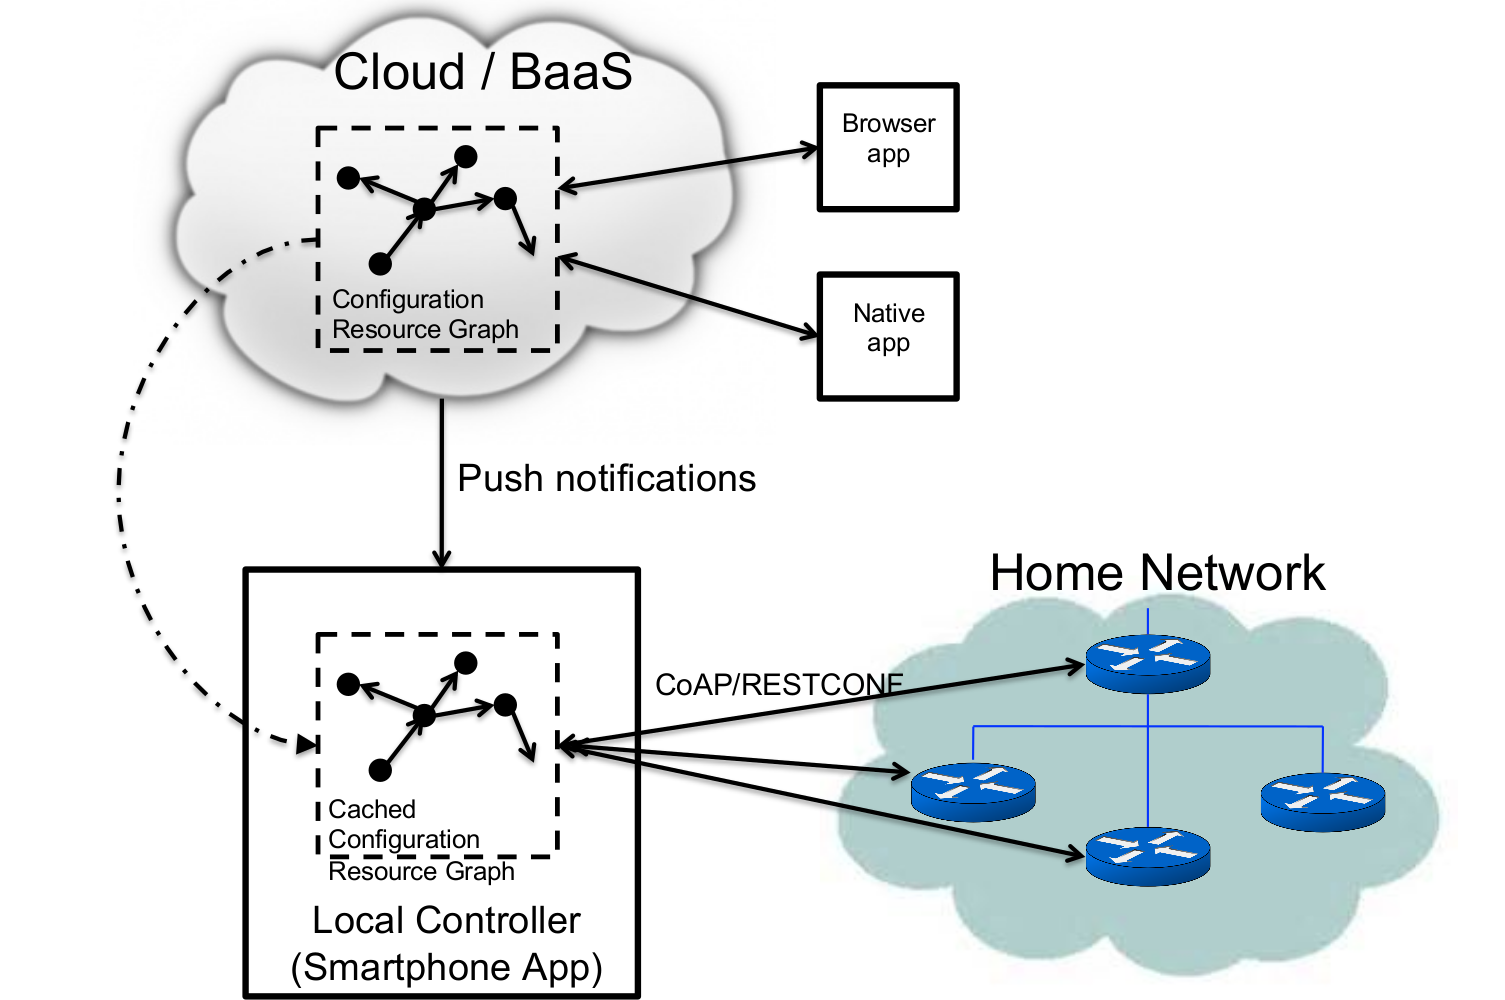
\includegraphics[width=.9\linewidth]{localcontroller.png}
\caption{\label{fig:localcontroller}Local Controller and Collaborative Management Design}
\end{figure}



The delegated service provider therefore does not need to have a direct data
access to the home but only to the cloud based service in order to be able to
manage the home network devices.
Consultant service is not the only possible delegation for home network.








One of the security issues is the authentication and authorization 
from the cloud to the home net.
To secure the connection from the cloud service (controller)
to the home network, there needs to be a mutual trust between the end
points, and the research problem here is how to enable the trust between the
controller and the home network as the controller lies at the edge of the
home network.


Any encryption between devices needs trusted key exchange beforehand,
and finding and establishing trust is needed for that.  That is called
the key distribution problem. Public and privat keys solve the key exchange part, but
only partially, because the trust still must be found somewhere.
The above mentioned cloud solution for delegated home network
management currently has preliminary authentication and access model
using pre-defined credentials and SSH-connection from the local
controller device to configuration
targets\cite[Chap.4]{silverajan2015collaborative}.
That does not yet handle the bootstrap of the infrastructure, 
i.e., the first trust is taken as given. 

The smartphone with its Subscriber Identity Module (later SIM) and an
existing key infrastructure to the mobile
network operator (MNO) would later eliminate the requirement for an
additional credential distribution. That issue is studied in this
thesis.  Although the smartphone provides alternative authentication
method with its SIM key, usual methods to authenticate still are plain
username-password combinations.  Those security issues must be solved
before delegation in the cloud can happen.



The trust can be derived from the facts that already are known.  
The ultimate trust can be achieved by verifying the trust chains 
until the chain reaches a trust anchor.
The trust anchor is the fact, state or place,
where derivation of trust is done no more, but accepted per se.
Combining existing techniques, this thesis presents one possible way
to bind the home network's trust to the smartphone's unique, existing
secret keys inside the smart card's Subscriber Identify Module (SIM),
which then would function as a trust anchor. 








The Human aspect and usability are important, but the focus will
still be on authentication and authorization part of the home net
management with smartphone as a trust anchor.  The proposed model
should nevertheless require less effort than the currently used methods
on distributing user credentials, finding the right place for them to be
inserted, and ensuring that they are written correctly.
Besides those, problems such as limited connectivity are
studied.





The thesis is structured as follows: authentication--authorization
model is explained in Chapter \ref{sec-2}.  Chapter \ref{sec-3}
describes security in current home net architecture and current
practices for configuring it.  Chapter \ref{sec-4} discusses methods
to bring a trust anchor in the home network and explains the chosen
method.
One specially crafted problem is how the scenarios presented here can be
tested without knowing the SIM card's secret keys and without real phone
operator involved.  Those experiments are described in Chapter \ref{sec-5}.
Results are discussed on Chapter \ref{sec-6} and Chapter \ref{sec-7} concludes the
thesis.
\chapter{Authentication, Authorization, and Trust}
\label{sec-2}



Authentication, authorization, and accounting services (AAA) are
components for access management.  AAA-protocols do not dictate
policies, i.e., who is granted access or what operations user is
allowed to do. They only transport this information between a client
who needs them and a server authorized to provide them.
Often, the last 'A' which stands for accounting has been neglected
and also here only first two A's are used and later described as AA
services. Authentication (AuthN) answers how to identify users and
prove that they really are who they claim to be. Authorization (AuthZ)
answers what operations the identified users are allowed to do and
forces usage policy. The rest of the thesis uses shortened terms AuthN
and AuthZ.

On very small environments AA service is built on a static backend such
as a file on a protected target that an entity wants to access. There AuthN
is checked against a credentials file and AuthZ from a service
specific policy file. 
To be more exact, the identification preceding the authentication is the part,
where the entity claims and presents its identity to 
access controlling system. That can involve sending username, login
name or other identifier. Authentication in turn is the part where
those facts are verified. AuthZ involves checking, which rights are 
available for authenticated entity. 


Before we introduce SIM-based authentication used throughout the
thesis, protocols 802.1X, WPA2, EAP and RADIUS are described in the
following Sections. [sections?]. Last, we expand the term \emph{trust}.

\section{802.1X}
\label{sec-2-1}

802.1X\cite{8021X} is an IEEE standard protocol for port based access
control. Ports are physical layer ports, not to be mixed to Layer-4 ports such as TCP/UDP ports.
 Network access through a specific physical port is
restricted (controlled) from a client (called Supplicant) before
the client has successfully performed an AA. A 802.1X device, where
the ports are located, is called an Authenticator. Third party in 802.1X is an
Authentication server. 



It is easy to mix here terms \emph{Authenticator} and \emph{Authentication
server}, but their roles are different: Authenticator works as a
gate-keeper to ports between supplicant and network, while
Authentication server handles the AA processes.
At home, Authenticator usually lies inside the access point, but 
on large enterprise networks, Authenticator may be a centralized unit 
and multiple access points function only as radio stations.



\section{RADIUS}
\label{sec-2-2}
\label{sec:radius}
RADIUS is the most popular provider for 
AAA-services\cite[p.75]{radius-popular}.  It was used first with remote terminal
and dial-up modem users, hence the name Remote Authentication Dial-In
User Service. Later it was used as centralized AAA for networking
devices such as switches and routers.  










RADIUS protocol is a stateless, request-response type client-server
protocol. 
There are four types of RADIUS messages defined in RFC2865 that are
used in AA. ACCESS-REQUEST and ACCESS-CHALLENGE cover both AuthN and
AuthZ messaging while final RADIUS message is either
ACCESS-ACCEPT or ACCESS-REJECT, based on the
result given by the RADIUS authentication server.

Today, RADIUS has some shortcomings and fixing them is not anymore
reasonable as developing has shifted to another AAA protocol called
Diameter, which is already in use in 3GPP and 4G
networks\cite{diameter}.  Nevertheless, as RADIUS is so wide-spread,
it is still used in lots of places instead of Diameter.  Currently,
the main environment of RADIUS, besides AA in network managing, is wireless
connections (Wi-Fi) in enterprises and nationwide community
federations.


When local Wi-Fi groups in Finland such as ``SparkNet'', ``Langaton
Tampere'', or ``Wippies'' started to form in around 2005, they used
802.1X and RADIUS for AA. Those networks did still have as an
alternative AA method a captive portal technique, where user had to
first authenticate on WWW-page before getting an access.  802.1X and
RADIUS brought an external, central RADIUS server for authentication
requests automatically, without burden of the captive portal.

The members of Wi-Fi groups could then use the network anywhere, where
the same uniform SSID (Service Set IDentifier) was seen, i.e., roaming
became possible, if one found a familiar SSID outside the home area.
Later, there were agreements between different local groups to allow
roaming and so federations were born.

As seen from federated Wi-Fi groups, RADIUS servers can be chained to
form a tree. The reasons for the chaining are load balancing and high
availability, centralization of locally distant servers, and
federation of different domains. In RADIUS trees, the messages are
can be proxied to next RADIUS server in the chain, depending on the settings
on the proxying RADIUS server.


In the following chapters it is discussed how proxying servers take 
part in AA decisions. Of main interest there is, if it is possible 
to inject or modify AuthZ information in those proxying RADIUSes in
cases, where AuthN and AuthZ are provided from different
 places\cite{rfc2607}. Secondary goal is to universally divide AA regarding 
client's domain in the federation.




\section{WPA2}
\label{sec-2-3}

Wireless protected access (WPA or WPA2) protects the traffic in a wireless,
shared media, where everyone otherwise can simple listen all the radio traffic.
It enables both authenticated access and message
encryption between a client device and  a wireless access point (AP)
by negotiating session keys. This happens 
after 802.1X has opened the virtual port in AP for the client.

WPA (version 1)  was an early subset of then upcoming 802.11i standard,
while WPA2 is the full implementation, also denoted as IEEE
802.11i-2004, and the term WPA2 is used throughout the thesis.
Client software for 802.11i is called a WPA2-Supplicant and it is used
in wireless clients to communicate with the Authenticator. 

WPA2 has two modes of protection: one for groups with common, pre-shared
key (WPA2-PSK, also known as WPA2-Personal) and one for individuals
having own key (WPA2-RADIUS, also known as  WPA2-Enterprise).  With WPA2-RADIUS, revoking
individual access is easier, but client setup slightly more
complicated than on WPA2-PSK, as seen on Table\ref{psk-enterprise}.

\begin{table}[htb]
\caption{\label{psk-enterprise}Comparison of WPA2-PSK and WPA2-ENTERPRISE modes}
\centering
\begin{tabular}{l|l|l}
Property & WPA2-PSK & WPA2-ENTERPRISE\\
\hline
suitable for groups & x & \\
suitable for individual &  & x\\
individual client revocation &  & x\\
client setup & easy & intermediate\\
\hline
\end{tabular}
\end{table}


\section{EAP}
\label{sec-2-4}

New AuthN methods are invented all the time.
Instead of implementing them into 802.1X, it was 
extended with a modular framework called 
 EAP (Extensible Authentication Protocol)\cite{rfc5247}. 
Researchers justify using EAP, as it
provides flexibility independent from underlying technology, whether
wireless or wired,  and integration with AAA infrastructures, although
it adds some overhead to AuthN\cite{pereniguez10}.
Different authentication methods, for example hashed passwords, TLS
 certificates, or SIM/AKA using smartphone's SIM card,  can
be used with EAP.
This work uses EAP-SIM authentication method.


EAP describes only the messaging form, so EAP messages needs to
be encapsulated inside another protocol.  In Wi-Fi, between a smartphone
and an AP, EAP can be encapsulated into 802.1X protocol (as EAPOL) or
into protected EAP(PEAP)\cite{peap} before sending
into air. In wired net those EAP messages are translated and encapsulated into RADIUS.

The encapsulation is described in Figure\ref{fig:eap-layers} where it can be
seen, that EAP messaging happens logically between the EAP peer and
the Authentication server. On a lower transport layer between them
there is an EAP Authenticator, which transfers EAPOL messaging into
RADIUS message.

Further, EAP is used to transfer AuthN messages only.
It includes neither AuthZ information, which is RADIUS's
responsibility nor session keys, which are negotiated by WPA2.  In the
end,
the Authenticator is the responsible for opening access for EAP peer as 802.1x
dictates.







\begin{figure}[htb]
\centering
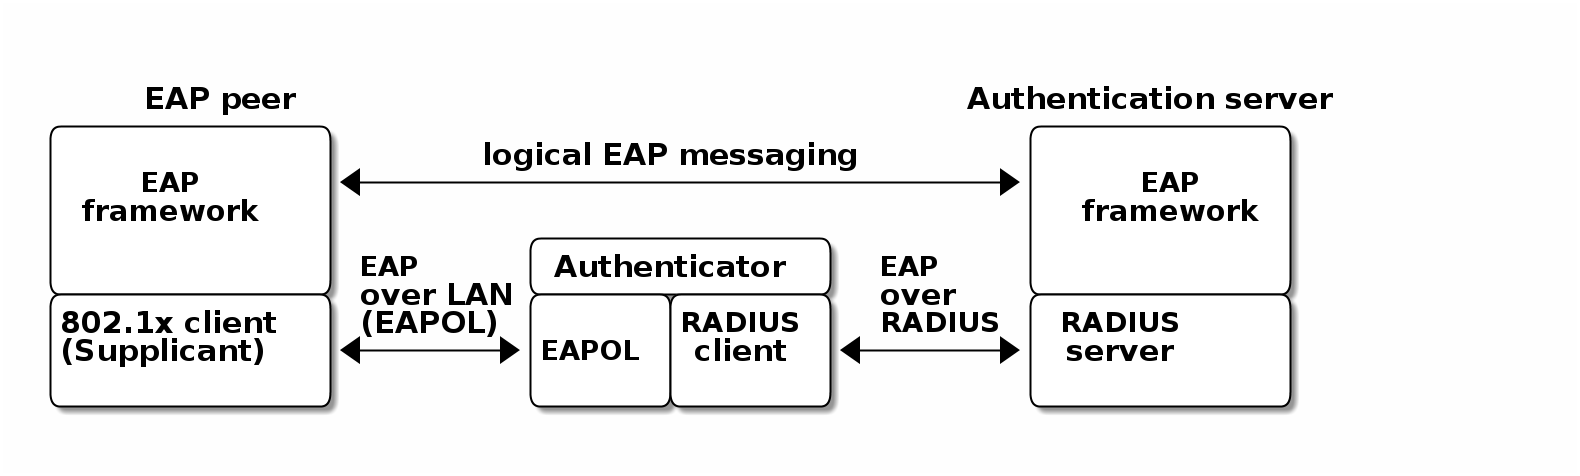
\includegraphics[width=.9\linewidth]{eap-layer.png}
\caption{\label{fig:eap-layers}EAP-logical layering and encapsulation}
\end{figure}



\section{SIM-based authentication}
\label{sec-2-5}
\label{sec:sim-based-auth}
SIM associates a physical card used in smartphones to
a subscriber of the Mobile Network Operator (MNO).
SIM here means the secret keys and the application in mobile phone's
SIM or USIM inside UICC(Universal Integrated Circuit Card).
The secret keys are hardware protected and only usable to applications
in SIM card.
The SIM's storage also includes a unique serial number ICCID 
(Integrated Circuit Card Identifier) which identifies SIM globally
and a unique IMSI (International Mobile Subscriber Identity). IMSI is
a composition of digits belonging to Mobile Country Code(MCC, 2
digits), Mobile Network Code(MNC,2-3 digits) and Mobile Subscriber
Identification Number(MSIN, 10 digits at most).
More familiar, it is the user's full international phone number.


SIM card usage can be controlled by two passwords: PIN and PUK.  PUK
is used as a remedy, if PIN has been inserted wrong too many times.
If the card has other applications, for example mobile electrical
signature application Mobiilivarmenne (see Section\ref{sec:altmethods}),
they may have different keys and codes.


The passwords, keys and cards are distributed by the MNO.
 and they 
provide the mobile network connectivity to customers of the MNO.  The
secret keys are used for authenticating the IMSI to MNO and that
enables MNOs to identify their customer in the network and charge them
correspondingly.  Client's identity is verified when SIM is delivered.
It is assumed, that SIM card represent its owner, but in reality
nothing prevents an identity thief to steal someone's SIM
card. Although the 4-digit PIN tries to prevent the usage of the
stolen SIM, that is considered weak safe\cite[p.31]{aaa-nakhjiri2005}.
The most important outcome of this distribution is the achieved trust
between the client and the MNO.


AA services need to trust some entity endpoint and in case of MNO and
SIM, they already mutually trust each other, and SIM can be used 
to open access to mobile networks.
Access to the Wi-Fi networks still needs a separate access credential
and that was the reason for developing EAP-SIM and later the
derivatives EAP-AKA and EAP-AKA'.  The goal was to combine 
existing keys used in  GSM (Global system for Mobile communication)
in a secure way to Wi-Fi access. Existing general purpose EAP-methods in 2004 were not
compatible with GSM protocols for this purpose.\cite[p.93]{hav-doc}
The results of that development gave us EAP-types EAP-SIM, EAP-AKA, or
EAP-AKA'(AKA-PRIME).

EAP-SIM is the original type created for GSM networks and defined 
in RFC4186\cite{rfc4186}.
It is a challenge-response method and similar to AuthN used in GSM, 
but it adds mutual AuthN, i.e., also the network is authenticated.
Beginning from 3GPP networks, new types EAP-AKA and AKA' can be used.
EAP-AKA is defined in RFC4187\cite{rfc4187} and 
uses 3GPP's AKA (Authentication and Key Agreement) protocol.
It adds to EAP-SIM additional parameters such as
sequence numbering from MNO to protect replay attacks and more
advanced digestion functions instead of SHA-1.\cite{rfc5448}.
Otherwise the protocol messaging is same as in  EAP-SIM.
Last, there exists EAP-AKA' that enhances AKA by including Service Set
Identifier (SSID) 
in the key derivation function, which limits the possibility of using possibly
compromised network's nodes and keys. 


  Using EAP-SIM means using the secret key inside SIM card with A3/A8
algorithms to generate valid responses for the challenges coming from 
MNO and to derive session keys.  The algorithms A3/A8 and their
possible implementations (COMP128, COMP128v2, COMPv3) are not of
interest in this work beside the point that they are MNO specific or known reference algorithms.


EAP-SIM variants provide strong AuthN which means here two-factor
AuthN. A one factor  is something you own (physical SIM) while  
another
is  something you know (SIM card's PIN). Biometric factor, i.e., what you are,
is not used here, but that would be a third different possible factor.
Software based certificates, while stronger than regular passwords,
on the other hand do not possess the properties \emph{non-copiable} or
\emph{unique}, so they can only be considered as strong passwords and 
do not full-fill the requirements for two-factor AuthN.  If we nonetheless
were using software certificates with a method such as EAP-TLS, then the
certificates (for CA and client) and the private key should still be
provisioned first, which would defeat what we want to achieve in
easy user experience.


Disadvantages with SIM are dependency on mobile operator and internet
connection, although disconnectivity issues are later addressed
partly in Section \ref{sec:disconnections}.
Using smartphone may cost money, either to client or to service
provider, but costs could be lower than using SMS, because 
the network  used is IP network instead of cellular phone network.

In many parts, SIM variants of EAP are simpler than other EAP
variants to mobile client.  Table\ref{table-peapsim} compares the setup of Wi-Fi
in clients of one existing organization to EAP-SIM. It
is noteworthy, that plain EAP-SIM will not support identity hiding and
that will be later discussed further. If we added PEAP
also to EAP-SIM (in last column of Table\ref{table-peapsim}), comparison would be more fair.
As can be seen from the table, leaving certificates out from the environment
makes client setup easier with the price of revealing smartphone user's
identity.  



\begin{table}[htb]
\caption{\label{table-peapsim}WPA2-Enterprise client setup with EAP-PEAP-MSCHAPv2 and EAP-SIM}
\centering
\begin{tabular}{|l|l|l|ll|}
\hline
 & EAP-PEAP & EAP-SIM & EAP-PEAP & \\
Task: & with &  & with & \\
(x)=``needed'', (N/A)= ``not available'' & MSCHAPv2 &  & EAP-SIM & \\
\hline
CA settings: &  &  &  & \\
- choose CA for the RADIUS & x &  & x & \\
- if CA-key not known, fetch \emph{securely} & x &  & x & \\
\hline
Other settings: &  &  &  & \\
- used EAP-method & x & x & x & \\
- validation of RADIUS server's name & x &  & x & \\
- encapsulation (WPA2/802.1X) & x &  &  & \\
- password & x & x(PIN) &  & \\
\hline
Identity hiding: &  &  &  & \\
- enable PEAP & x & N/A & x & \\
- outer identity & x & N/A & x & \\
- inner identity & x & N/A &  & \\
\hline
\end{tabular}
\end{table}

\section{Analysis of EAP-SIM protocol}
\label{sec-2-6}
Bird's-eye view to the EAP-SIM protocol messaging between the
smartphone, AP, Authentication server and MNO with its Home Location
Registry Authentication Center (HLR\_AuC) is described in
Figure\ref{fig:eap-sim-bird}.  The traffic is EAP on the left, RADIUS in the
middle, and MAP/SS7, which is an mobile connection application running
over signaling system (SS7) used in cellular networks, on the right.


\begin{figure}[htb]
\centering
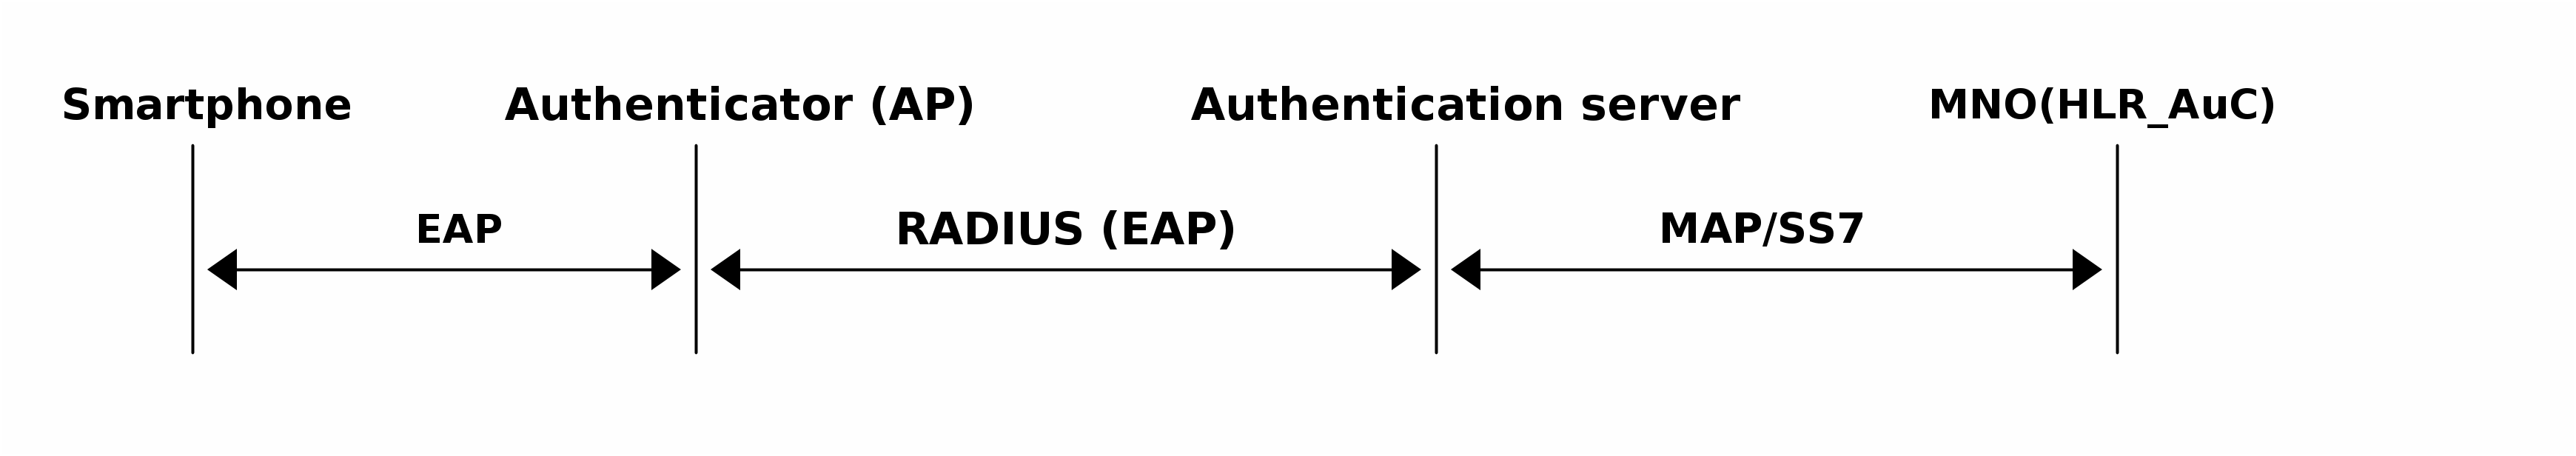
\includegraphics[width=.9\linewidth]{eap-sim-bird.png}
\caption{\label{fig:eap-sim-bird}Bird's-eye view to EAP-SIM components}
\end{figure}





Protocol analysis of full EAP-SIM authentication is described 
in Figure\ref{fig:eap-sim-radius}.
Important parameters for this work are IMSI, NONCE, and triplet values
RAND, SRES, and Kc. 
From traffic between Supplicant (here smartphone) and Authenticator (in AP)
we can see that IMSI is used first in message 3. IMSI is the
identity, which Authentication server would next try to challenge as
part of the AuthN and for which the AuthZ would be checked.







All EAP-SIM derivatives provide mutual authentication.
An operator (network) is authenticated with help of a nonce,
which is by definition ``number used only once'' and can
be thought as a client's challenge to the network.
The nonce is transmitted in the message 7 in Figure\ref{fig:eap-sim-radius}.
The client later checks in the process 13, whether RAND values from
the operator were digested with the correct nonce and so authenticates
the operator.

The client in turn is authenticated, when the Authentication server
generates a challenge with an aid of a triplet from the MNO and the
client responses to the challenge correctly after processing it with
its own \emph{Ki}.  Correct answer would be SRES which the Authentication
server received in message 10.
\begin{figure}[htb]
\centering
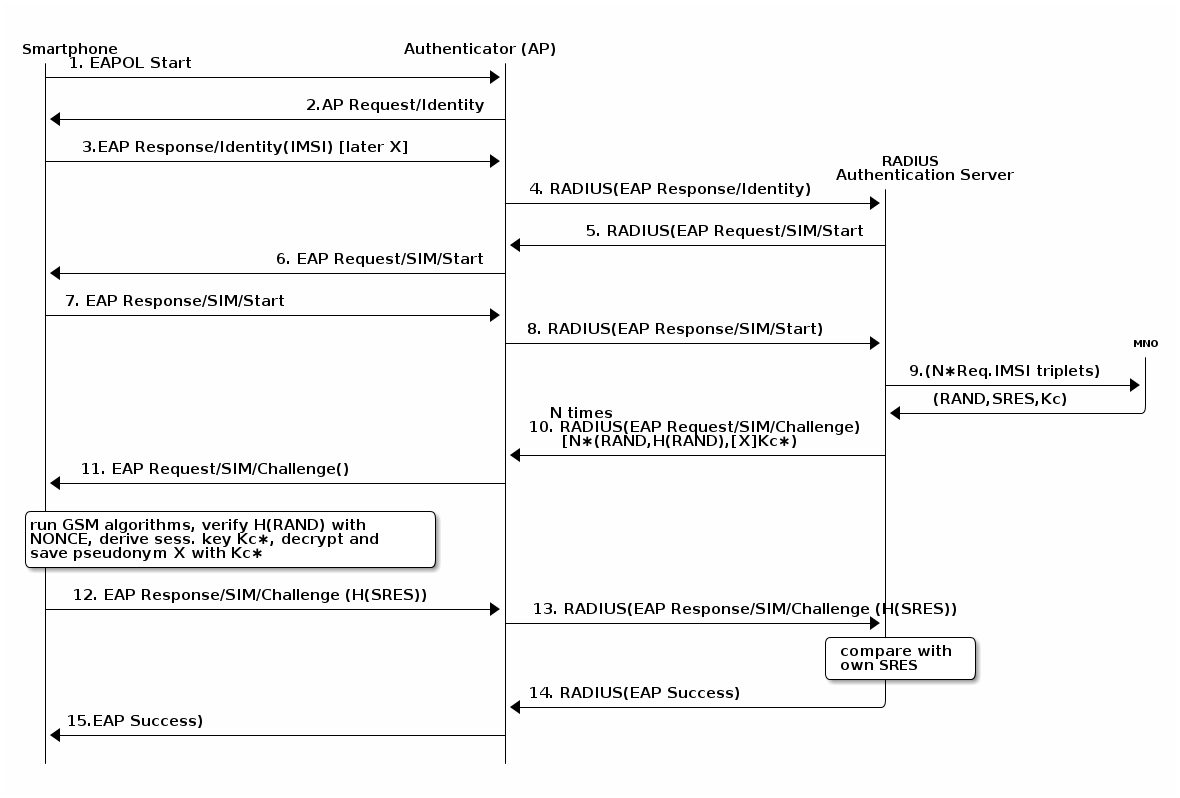
\includegraphics[width=.9\linewidth]{eap-sim-radius.png}
\caption{\label{fig:eap-sim-radius}Successful EAP-SIM full authentication with RADIUS}
\end{figure}



After mutual authentication, the AuthN phase has been completed. The
Authentication server completes the AuthZ by sending the Authenticator either
an Access-Accept or Access-Deny RADIUS message. 
Accept message triggers 802.1x protocol to open a virtual port in AP
and lets the WPA2 process continue in exchanging WPA2 session keys. 

Both parties have now retrieved the same trusted key \emph{Kc}. The
Authenticator has received it directly from RADIUS message 10 and the
smartphone has generated it using its own secret \emph{Ki} key in
process 13.
Therefore the derivation of secret session key for WPA2 is possible.

After the session has been set, IMSI may be left out and a temporal IMSI
(TMSI) can be used instead to hide client's identity, for example in
fast re-authentication case to reduce the risk of exposing the client's
IMSI unnecessarily. Unfortunately, at that point, IMSI has already
been exposed at least once in plain text, namely in message 3.

TMSI is composed of a pseudonym and a realm part and can be a
string. So, one can send 
\texttt{my-string-which-can-change@…operator.domain} instead of 
IMSI number as an identity. 
It must be noted, that TMSI used here differs from TMSI used in 3GPP
networks. Those context must not be mixed, otherwise the security that
they bring may decrease, i.e. one must not use the TMSI received from
3GPP as TMSI in EAP-SIM.
\section{Trust}
\label{sec-2-7}

Secure communication has many layers and on its base lies trust. 
Only after completing trust setting phase it is meaningful to complete
the other security layers. For example, secret keys enable encrypted
communication, but they need to be delivered first through an trusted
channel. Same applies to public key infrastructure solutions, when
verifying the public keys and so it can be seen that trust
really is the first layer to be fixed.



Even without trust, some form of secure asymmetric key-exchange is achievable
with Diffie-Hellman key-exchange\cite{diffie1976new}. Unfortunately, it is vulnerable
to Man-in-the-middle(MitM) attacks, where the protocol does not notice, 
if messaging has gone through a third party, which impersonates itself to 
both ends as being the corresponding messaging partner. MitM can
read and decrypt encrypted messages and forward possibly changed message with
a correct looking signature.
With trust set between two devices, i.e.,  if they can securely
authenticate each other, secret communication is possible. 
Secure network configuration and credential exchange is then possible.


This trust can be used to include other components under the
same trust circle in the home network. As mentioned earlier, the SIM
and MNO trust each other hence mutual authentication between them is
possible and that is later shown to be an important factor.  Also the
key distribution problem mentioned in Chapter \ref{cha:intro} is solved
already at SIM-card distribution phase.  As AuthN-AuthZ at home
proceeds through the Authenticator, then the Authenticator must
deliver this information further and use it as a derivation function
to extend trust.




\chapter{Home network architecture}
\label{sec-3}

\section{Home network architecture and IETF}
\label{sec-3-1}


While home network is any network located at person's home consisting
of devices and their connections, either wired or wireless,
this thesis avoids using term \emph{homenet} when meaning those networks
because  homenet  is  reserved to 
Internet Engineering Task Force Working Group's (IETF
WG) homenet. IETF is responsible for the most internet technology standards and 
WG homenet was started in year 2011.
Current drive in homenet management is towards IPv6 environment
 as it allows future addressing and routing needs. 
Homenet has five tasks to solve at home networks: service discovery, network security, 
prefix configuration for routers, routing management and name
resolution.\cite{homenet-charter}.
As old technology cannot be forgotten, home networks will be heterogeneous having both
old and new technology, and their interoperatibility is important in
planning future home networks. 
Segmenting home in multiple subnets will also belong
to homenets and will include areas for home members, guests,
and management. It will not be so uncommon to have a cheap second
network operator for backup purposes at home, so issues about
multihoming are added to homenet.
Lastly, end-to-end access, is in their
agenda. End-to-end access, i.e., restriction-free access was the key
element for the internet's success and it enabled many new
applications in the past, but has then had difficulties because of
firewalls and NATs.



Securing home network and its router's configuration can be done for
example first limiting access to their administrative ports
with static or dynamic extended access control lists (ACL) in
routers. To get through administrative ports, i.e., to login and make
configuration changes, there exists either AAA or local authentication.
Authorized agents can then make changes, either direct in the device or through some
management protocol such as SNMP or NETCONF[source needed?].  SNMP has been in
use for over 30 years and is well supported in routers. Yet there are
multiple version for this protocol. While earlier versions (v1, v2)
did not provide any encryption of messages, version 3 knows for example
about public keys and is secure enough when used correctly.


Customer Premises Equipments (CPE) such as ADSL broadband routers or
set-top boxes, connect customer's network to operator's network.
Management of CPEs on the border of home network and operator has 
existing protocols. For example, TR-069 standard\cite{iptvtr069} for CPEs
has been used to implement self-configuration archi\-tecture in
home networks\cite{tr069rachidi2011}.


RFC7368 about IPv6 Home Networking Architecture Principles from
Arkko\cite{rfc7368} defines the borders of the home network and states that
internal borders in home network should possibly be automatically
discovered. Limiting those borders to specific
interface type would make it difficult to connect different realms locally.
The same document continues stating
that while home network should self-configure and self-organize itself as
far as possible, self-configuring unintended devices should be
avoided and let home network user decide whether device becomes trusted.
So, these statements reveal us that home network environment still needs
external configuration even with the proposed automation aids.

\section{Centralization trends in management}
\label{sec-3-2}

Traditionally, configuration management of network devices has been done
individually using each device's console or web-access.  As the number of
devices has increased, it would have been reasonable to rationalize
the process by utilizing a central management, not least to prevent human
errors for repetitive tasks.  The reason, why this has not happened at
home, is because network devices there often are too heterogeneous, bought at different times from different vendors
and therefore incompatible with each other and.

To help in moving the management to a more centralized
model, the home network will see smartphone as a central managing local
controller.
Usually, home users already have a phone, which can be considered 
`smart'. Most smartphones have Wi-Fi capabilities and writing programs
for them is possible even with only little knowledge.
When we choose a smartphone to be the management point, the other benefits are
numerous:  a management software can be delivered and
updated from cloud to diverse smartphone types, existing user
base having smartphones is orders of magnitude more than in any single
organization, and as the most important fact, the trust anchor can be set to the smartphone.

The users already are  centrally located  in operators' user databases
in HLR-AuC.  To achieve the management paradigm change to a central configured one,
we still need to bridge the+ home network to that model with a trusted local controller
and then resolve the work-flow of change management.


Home Network change management itself is mostly excluded from this work.
For example, 
it is desirable, that changes in home network are done only through
local controller, not at local device because of
synchronization issues, even 
if synchronizing algorithms such as Trickle\cite{rfc6206} were used in
home network for configuration propagation. As another example,
configuration also includes
power level settings of devices to save electricity based on usage
profile. For example at nights or when there is nobody home, some
devices do not need to be working at their maximum capacity, and
details of how this scheduled is out of scope.

Instead, we study interfaces of AA.  Main points here are an existing
infrastructure (phones, internet access, Wi-Fi access points),  a strong
authentication (two-factor), and authentication methods
(EAP-SIM, EAP-AKA, EAP-AKA').

\section{Methods for introducing trust anchor into the home network}
\label{sec-3-3}
\label{sec:altmethods}

 Trust information, may it then be a secret or some
other evidence, can be delivered to a trust device via physical
transport channel separate from the actual communicating channel.
Traditional way to do that is with a password inside a sealed
envelope or a one-time password list that for example online banks 
use today. The secret can also be sent as an SMS.

In this thesis,
the phone brings trust to the home network by completing a full EAP-SIM
AA through the local Authenticator. SIM's identity is verified by HLR
AuC at the phone operator's end and AuthZ added to it later. The
verification leaves a trail on the local Authenticator and opens a
trust channel for a limited period of time for changes from the phone.




Trust can also be requested with help of device's unique
properties. Recently, devices have appeared on the market, that have
vendor provided certificates inside them and this brings public key
infrastructure as one possible alternative for learning trusted
identity.  The device proves its identity by presenting a certificate,
which has been issued by a trusted vendor and which includes devices
public key.  Private part of a key pair is inside the device's trusted
hardware store and does not ever leave the hardware. Vendor trust is
needed for checking the issued certificates and so the trust
verification of individual devices is merely transferred to trust
verification of the vendor.  Root CAs are trust anchors also and can
be read in the same way from the device's read-only store.  CPE could
use vendor issued certificate for AuthN of some earlier unknown
device.


Other techniques  to use SIM's unique properties besides EAP-SIM
are for example Bluetooth SIM Access Profile(Bluetooth  SAP), 
direct connection through PC/SC (Personal\- Computer/Smart\- Card),
CallerID service from phone network, or
Mobile signing service.
Bluetooth SIM and PC/SC would need patching of smartphone's software
to work.  On the other hand, the smartphone would any way need to
download  a controlling application
in the beginning for advanced use, so these techniques could be
studied further in another work.

Caller ID as an authentication method uses cellular network's controlling
channels. When a phone makes a call, the receiving end gets 
to know callers phone number (IMSI) before it answers the call.
That information is called Caller ID and it has been in use
successfully for some door locking implementations. 
It does not cost anything for caller or responder,
because after receiving the CallerID  information, responder can hang
up upcoming call and no call expenses are created.
 It can also be made safe at least in Finland
by limiting which tele operators are allowed to connect.














SIM card can also benefit from electronic signatures.
European Telecommunications Standards Institute (ETSI) has defined a
standard for mobile signature services (MSS) in ETSI TS 102 204.
MNOs in Finland have diverse implementations for this. The universal 
service is called ``Mobiilivarmenne'', but MNO Sonera's brand for it
is ``Sonera ID'' while MNO Elisa calls it ``Elisa Mobiilivarmenne''.

When AuthN and AuthZ comes from outside, one possibility is to use a
federated Mobile AuthN Service, which then is connected to  MSSP(Mobile
Signature Service Provider) with ETSI-204. Benefits for ETSI-204
federation are similar to those with federation of WiFi groups
mentioned in Section \ref{sec:radius} -- no home device must implement it at home,
but also beneficial for  MNO as it sees the service as just one
client.  Without the federation, the mobile AuthN services would need to be
multiplied with number of the separate home networks  needing authentication service.



Project Moonshot\cite{moonshot}, is in its early phases. Its goal is
to enable federated access universally to applications and
services. If it worked and was used together with MSSP, it may offer
SIM-based SSH access to Authenticator. Modifications are then needed 
both in SSH server and client. Additionally, EAP must be used through
tunneling, for example as an inner protocol of EAP-TTLS.

At this point a question might rise, why these external service
providers are needed. Is it not easier and simpler to just send 
an SMS with password code to the smartphone, when access confirmation is needed?
Mobile SIM provides two-way AuthN part as discussed earlier.
Without need for strong AuthN, that model would indeed be 
simpler, but using SIM also solves initial key distribution problem.
Additionally, mutual AuthN problem would still need to be solved:
Who sent that password and where that password should be inserted?





Requirement for home network can be as small as having WPA2 Enterprise capable
AP. Almost any AP will do, but as an exception, cable modem Bewan, which 
has been distributed to many homes from the cable modem operator Elisa, was found to have only WPA2-PSK mode.
Additionally, managing user's SIM-card has to be registered as an admin user in home network 
configuration, i.e., IMSI must belong to the admin group.
In this implementation, no extra application is needed in smartphone
for primitive trust, but later for more serious use some application is needed.
For added functionality, for example for logging admins out, OpenWRT
based software can be used, although those functions have not yet been
implemented. Disconnection issues are explained in Section
\ref{sec:disconnections}.




\chapter{Design of home network trust anchor and separation of change management}
\label{sec-4}





This chapter describes, how the smartphone becomes a trust anchor for
the home network and how the change management can flow after that.
On its simplest, the smartphone connects with a Wi-Fi link to an
AP in the home network and authenticates with SIM-card.
The resulting authorized connection brings a trust relationship
between the smartphone (a local controller)
and the home network (managed devices) so that the 
management can happen. 
In essence, the precence of the smartphone at home
opens the gate for the management, though it needs a little
interaction on behalf the user.



Before fully explaining our chosen method, we introduce some 
alternative
approaches for a trust anchor. The trust anchor is part of bootstrapping,
which is needed because although the smartphone and MNO
already trust each other, the trust between the smartphone and AP, and
thus the management network at home, is non-existing in the
beginning as can be seen from Figure\ref{fig:trustbegin}.

\begin{figure}[htb]
\centering
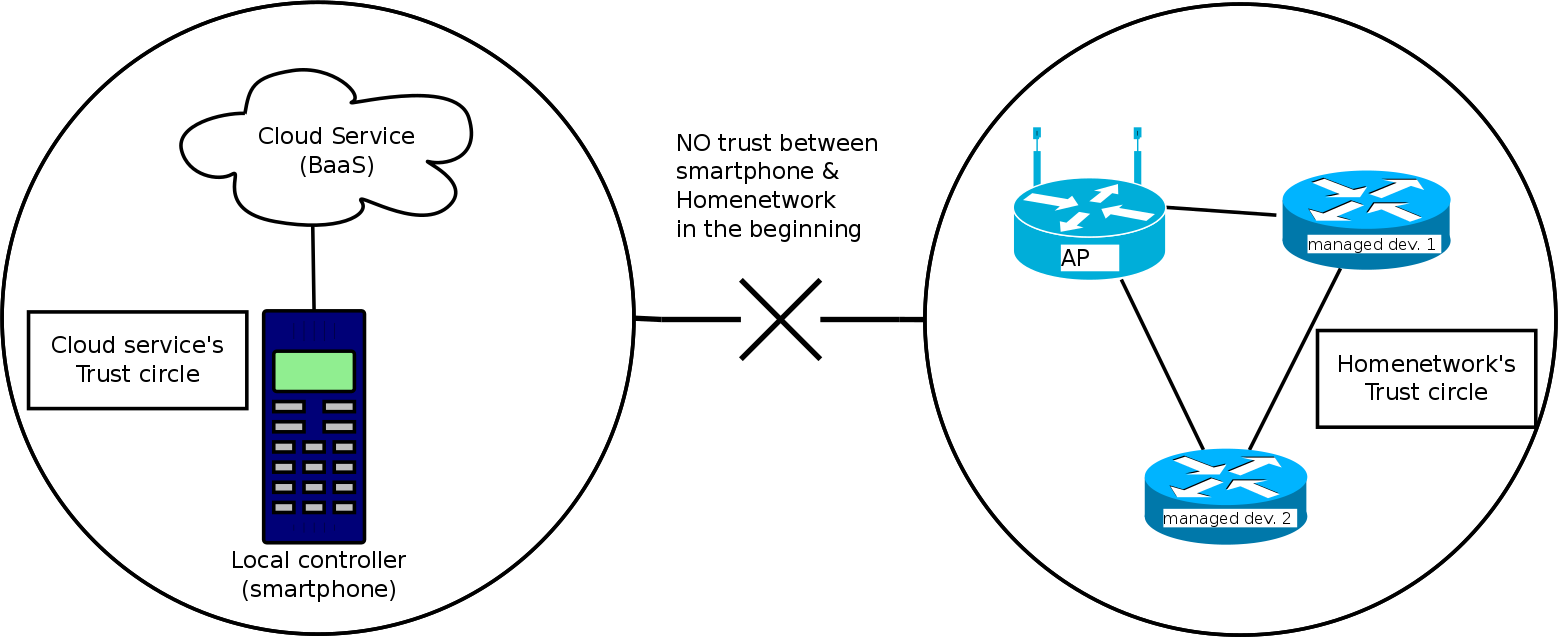
\includegraphics[width=.9\linewidth]{trustcircles.png}
\caption{\label{fig:trustbegin}Trust circles in the beginning}
\end{figure}


\section{Chosen AA design}
\label{sec-4-1}
\label{sec:chosendesign}



Network can be divided into separate segments based on user's role and
needs, such as guest or home members segment. The segments provide
base connectivity layer and simple separation. Different
services, like disk storage, can force their own policy on application
level.
It is not defined here, if the segmentation is made 
physical or virtual (VLAN, Virtual LAN). 
There is also a segment for devices management. 
An analogy to the real world would be public access corridors and doors for
customers that are separate from privileged doors for service personnel.


Routers control access to the segments with aid of 
access control lists (ACL), where decision is made based on current configuration or user's
role.  Once user has been authorized into management network, access
stays open for him, at least for a (predefined) limited time.

So, instead of checking user's credentials each time data is received,
this model only checks, from where data is received. 
Data received from the management network is granted for changes.
It is arguable a lighter method than always
fully AuthN and AuthZ but may suffice here, at first.



Example of a complex solution would be a traditional firewall and packet
inspection in the interconnects, but very modern model
is the de-perimeterization trend set originally by Open Group's
Jericho Work Group in 2004, that won't leave trust verification to
perimeters of network (firewalls and application proxies) but 
always handles traffic as coming from untrusted source.\cite{jericho2004}
One implementation of de-perimeterization is 
Google's BeyondCorp\cite{2014-beyondcorp}, 
where traffic always travels through Access Control Engine
and is suspected as being external, even when it originates from
inside networks. 




When home network needs secure binding to the smartphone, earlier
mentioned trust is the first one needed.  The trust is achieved by
checking whether the smartphone can access home management
network using only its trusted SIM-card, which provides AuthN. AuthZ in
turn is compared to existing roles of IMSI in the Authenticator.




When AP forwards authentication request to the next RADIUS server, it
can ask or receive, beside AuthN and AuthZ, other service parameters,
such as provisioning. RADIUS can carry those extra attributes in its
ACCESS-ACCEPT message.  In essence, AuthZ part itself can be thought
as one type of service provisioning.  That would then allow the
smartphone to connect to a specific management network and access the
devices either via command line interfaces, SNMP, or
similar\cite[p.4]{rfc5608}.
There exists RADIUS attribute types for directing user into specific
VLAN. If those do not suffice, there is also special Vendor Specified
Attributes (VSA). VSAs allow vendors to define up to 255 own
attributes that can be used in provisioning in homogeneous environment. 


That way (3rd party) Authentication server can decide which network
segment the device would be put.  In our case, admin users are put in
to the management network.  Yet, usually RADIUS ACCESS-ACCEPT message,
which means AuthN and AuthZ were successful,  puts the user in
default network, i.e., just gives it basic access. As for other
provisioning parameters, not all end devices support them.

In the first prototype it is enough to identify an authorized
smartphone's SIM.  Smartphone holding the SIM is granted the access to
the parts of the management network and it is authenticated strong.  User
management is outsourced to MNO, which
already has provided SIM cards to users. What remains, is the adding
of the user's IMSI to the authorized users' list. That list can be
located on diverse place, as can be seen in Section \ref{sec-4-2}.


After authentication and authorization has succeeded, session key
creation occurs (WPA2 session) between AP and the smartphone. 
The Authenticator has opened port to the smartphone for
configuration changes. 
The Local RADIUS (if existing) and AP have trail of a successful
authentication and know which IMSI has successfully authenticated in
the home net. They also know the mapping between IMSI and temporal TMSI for
cases when the smartphone later would need re-authentication.


Eventhough, the AP now has authenticated the smartphone user, the managed devices still 
need to have their own access control.
They may consult local RADIUS server, which tells whether there currently is an
authenticated smartphone present and then the changes going
to the management network would be allowed. Smartphone also could have
the login credentials to devices through earlier received
configuration information and use them after getting into management
network. This AA would happen on upper, application layer (layer 7), while
802.1X happens already on media layer (layer 2).

\section{AA component location scenarios}
\label{sec-4-2}


The AA components can be found in diverse location combinations. Here, the AuthN component 
usually is located outside the home, as MNO is the AuthN, unless
we are considering offline AuthN or recurring AuthN.
The AuthZ may be placed more freely. It can be at
home, at an external provider, or at MNO.
Authenticator on the other hand must lie at home, and 
gives the final decision about the access.

If the AuthZ decision is made on remote AuthZ server, 3rd party, 
then that server needs to have either local data or access to 
cloud service's AuthZ data (scenario III, external AuthZ).
Further it seems inevitable, that just like the home network model
in the cloud has  AuthZ data of eligible IMSI accounts,
then also delegating AuthZ function to the cloud would simplify home network 
management. Instead of putting logic on CPE for AuthZ, CPE
could just trust the 3rd party service's AuthZ message, which in case
of RADIUS is either \emph{ACCESS-ACCEPT} or \emph{ACCESS-REJECT}.


[Put the table maybe after the scenarios?]

Table\ref{table-scenarios} represents the locations for Authenticator (AA),
AuthN, and AuthZ in five scenarios. The locations are marked as (i)
for internal or (e) for external in the table and the scenarios are
described after that in detail. Authenticator is the entity which
gives the final decision about access regardless of location of AA
and it is always internal, located at home network.

\begin{table}[htb]
\caption{\label{table-scenarios}Location of AA, AuthN and AuthZ in scenarios I-V}
\centering
\begin{tabular}{lll}
scene no: & AuthN & AuthZ\\
\hline
I & e & e\\
II & e & i\\
III & e & i/e (proxied)\\
IV & i & i\\
V & - & -\\
\end{tabular}
\end{table}
\label{scenario-i}
The first AA-scenario is presented here thoroughly as an example.
The goal is to make a trusted configuration change. 
The steps are numbered and explained in detail in Figure\ref{fig:scenario-I}.
The configuration change is allowed, if CPE gets ACCEPT message from
MNO. Allowed users have been inserted earlier to MNO from the Cloud.


\begin{figure}[htb]
\centering
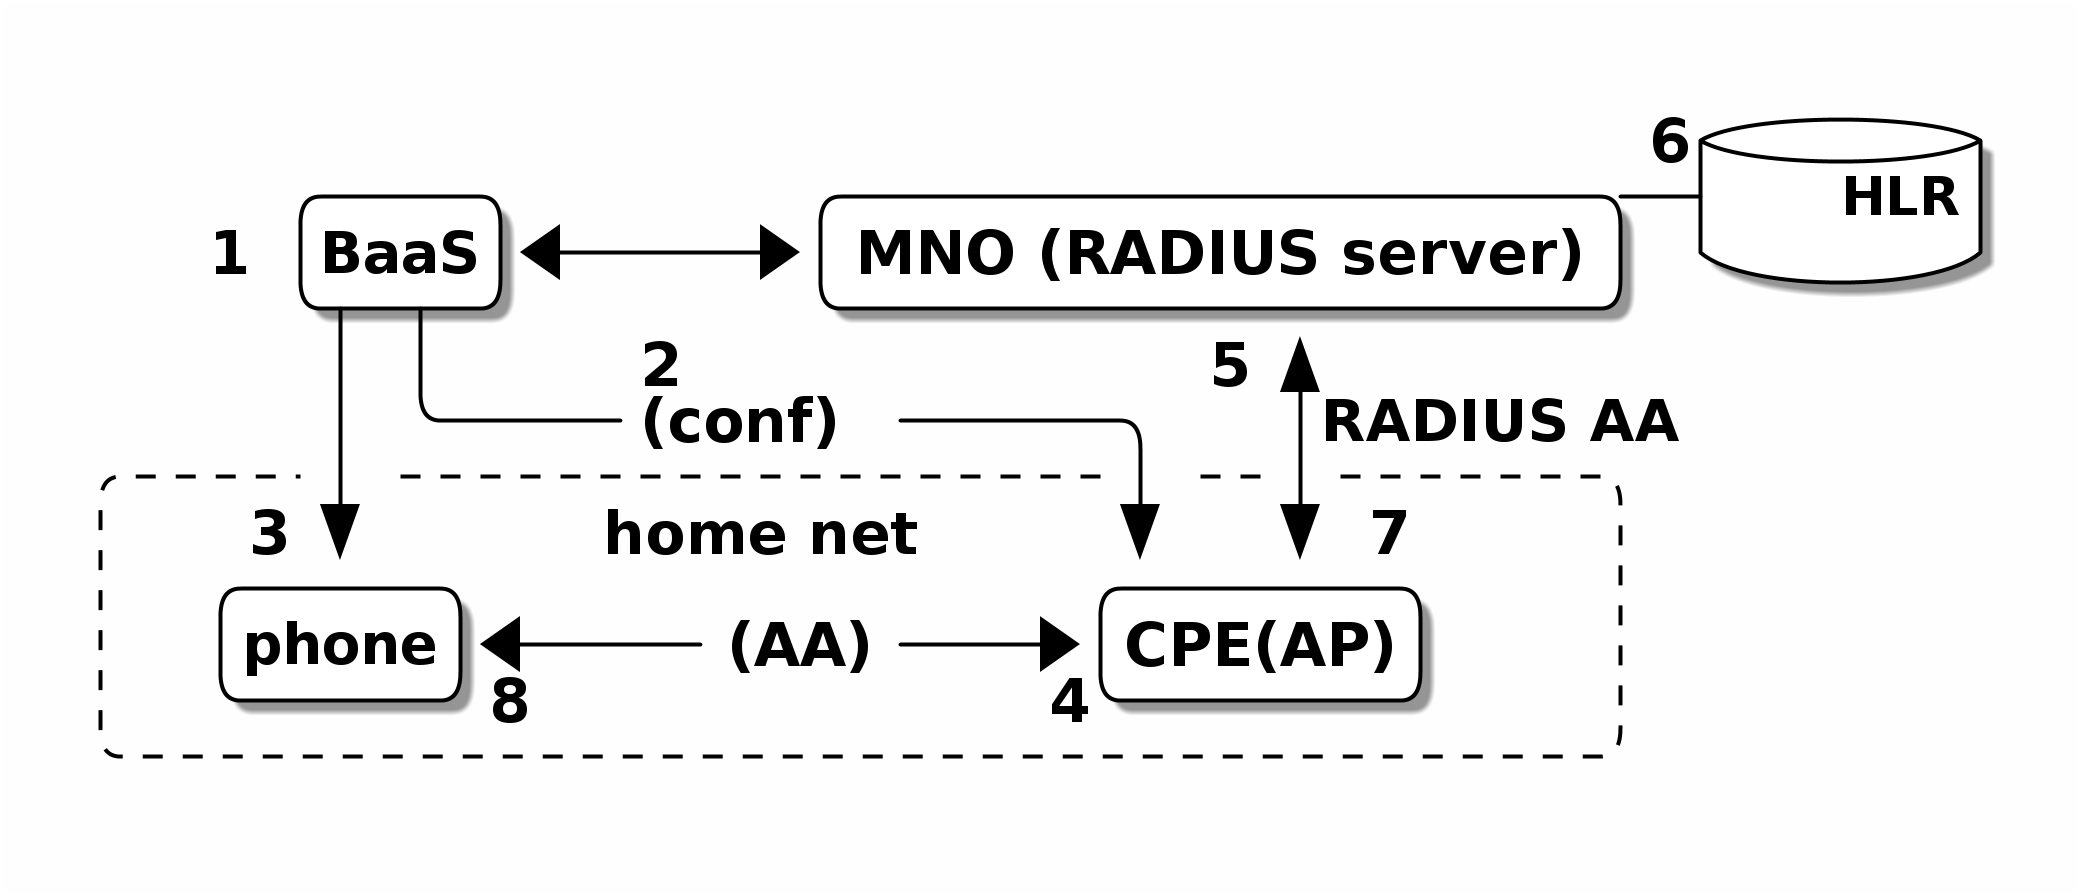
\includegraphics[width=.9\linewidth]{scenI.png}
\caption{\label{fig:scenario-I}General scenario I with 3 separate domains: Cloud, MNO and home net}
\end{figure}


\begin{enumerate}
\item The model has been changed in the Cloud.
\item The Cloud send the changes to the Local Controller (phone).
\item If the changes are privileged, they need to be approved by the phone user.
The phone user must  authenticate to the management network.
\item The phone user starts the authentication process to management
network using EAP-SIM and reveals its IMSI.
\item CPE (AP) forwards the authentication to MNO's RADIUS server using
RADIUS protocol.
\item MNO has RADIUS server which uses HLR-AuC for authentication
  triplets. 
  (AuthZ). This RADIUS continues the authentication process until to
  the end. 
MNO also asks from the Cloud, whether IMSI user has an admin role.
MNO returns in RADIUS message either \emph{ACCESS-ACCEPT}, if user is both
  known AND has admin role  or \emph{ACCESS-REJECT} if either property
  fails.
\item CPE receives this ACCEPT or REJECT. If there were other RADIUSes
between CPE and MNO, they would have acted
as proxy RADIUS servers.
\item IF ACCEPTed, then the smartphone is both authenticated and
authorized and it now 
can send configuration change message to CPE, which recognizes it
coming from authorized  network.
\end{enumerate}







\label{scenario-ii}

In second scenario (Figure\ref{fig:scenario-II}), AuthN is asked from MNO but
AuthZ is checked from local database. Local data comes from data model
i.e. from configuration data and will be saved in CPE, or some other
place within home network.


\begin{figure}[htb]
\centering
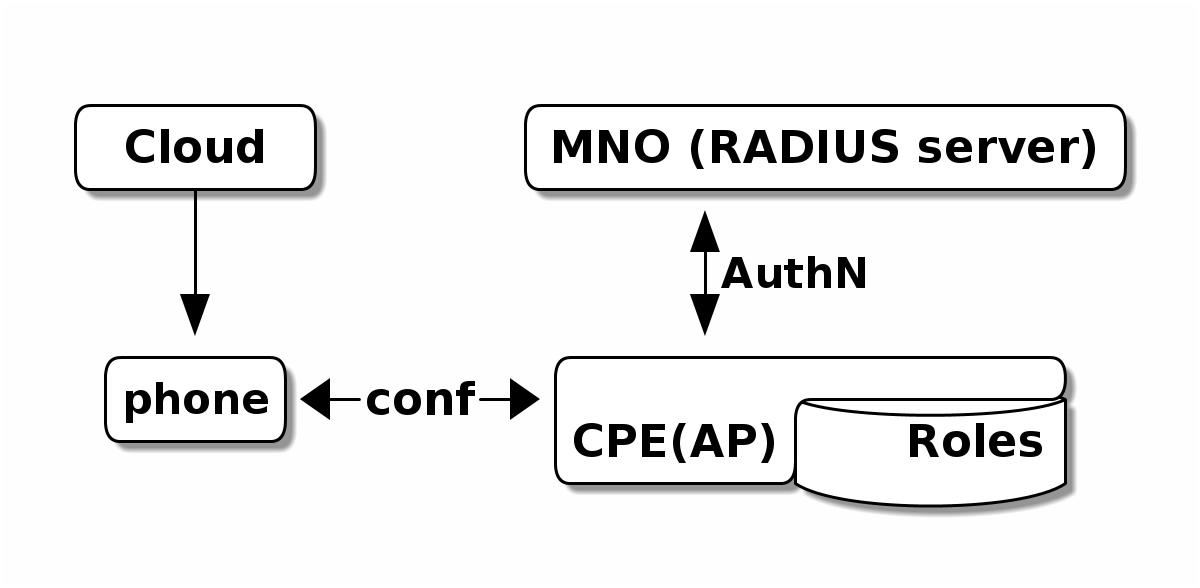
\includegraphics[width=.9\linewidth]{scenII.png}
\caption{\label{fig:scenario-II}Scenario II with AuthZ in home network}
\end{figure}


\label{scenario-iii}

Similar to first scenario is scenario III (Figure\ref{fig:scenario-III}), 
but this time there is a service provider between CPE and MNO, so AA is fully outsourced:
local AP communicates with RADIUS protocol to the external
Authentication server. That in turn gets AuthN from MNO via its own
HLR-AuC gateway and AuthZ from the cloud. It can also use alternative
sources for AuthN.
Locally there is a cache for roles in case of network disconnectivity.

Here benefit is, that 3rd party Authentication server may have direct
contracts to many alternative MNOs, so the user is free to choose its
MNO operator. As a bonus,  MNOs already delegate requests to right operator, if
they happen to get AuthN request which does not belong to them.
This is similar to federated service.

\begin{figure}[htb]
\centering
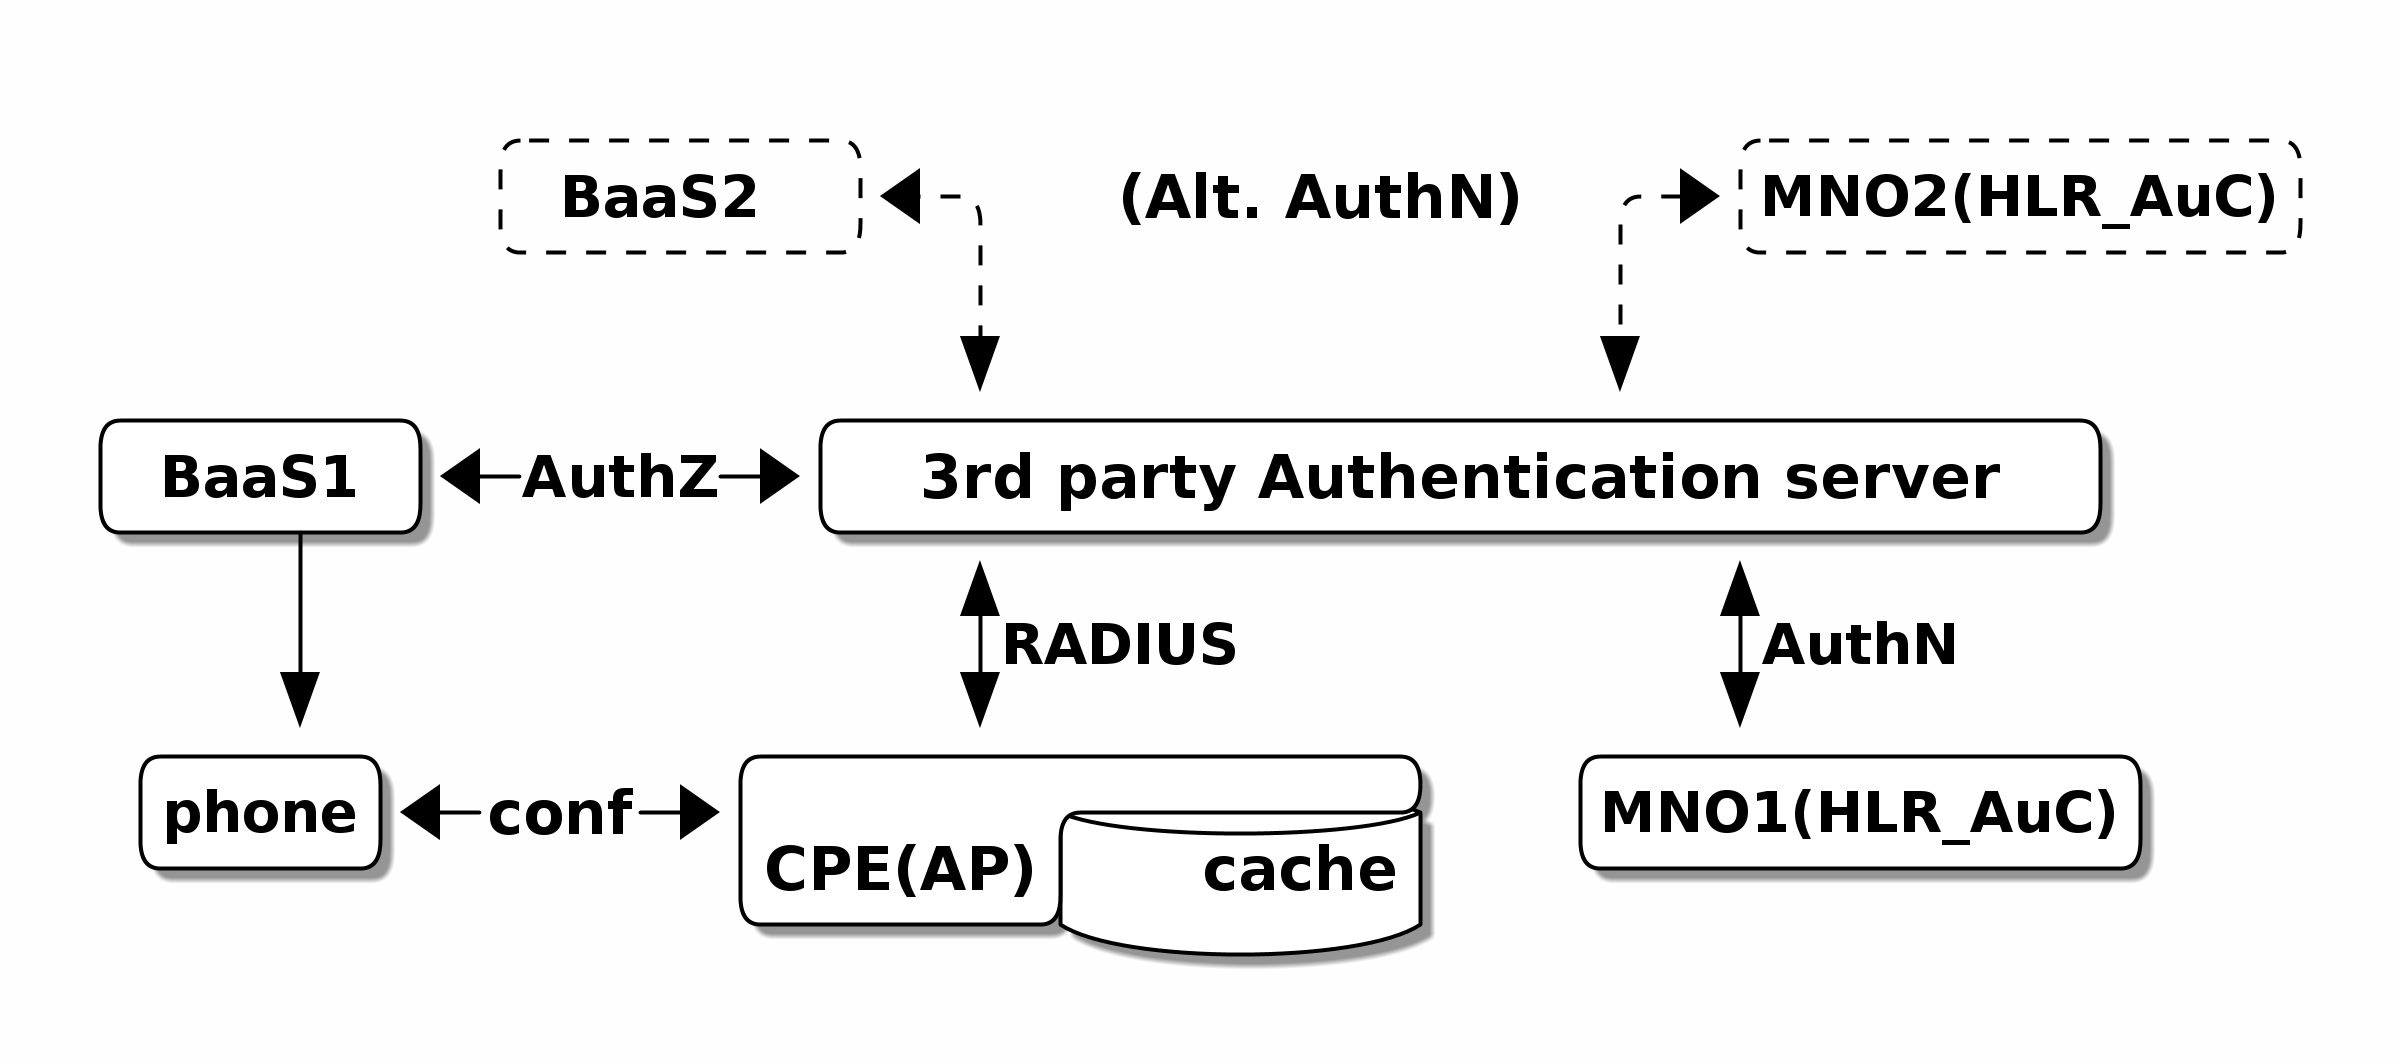
\includegraphics[width=.9\linewidth]{scenIII.png}
\caption{\label{fig:scenario-III}Scenario III with outsourced AA and backup cache for AuthZ}
\end{figure}

Allowed users are verified from the cloud's registries and specific IMSI is
authenticated from MNO.  It may need some preparation, if SIM
identities are temporary i.e. TMSI is used.  Still, IMSI is carried out at first message
of full authentication. Later, the server would need to have mapping
between IMSI and TMSI, but because only full-authentication is used,
there should be no problem.



If internet connection is down, local AA is still possible.
Full authentication uses IMSI, 
which is the identity of the phone's SIM.  Lighter, fast
re-authentication would use temporal identity TMSI. It can change
each time the AuthN request had been sent. Mapping of TMSI is cached
on the Authenticator and the round-trip and handling at HLR can so be
eliminated. Re-auth also works when there is no internet connectivity,
but Full authentication would not work because of missing MNO.


\begin{figure}[htb]
\centering
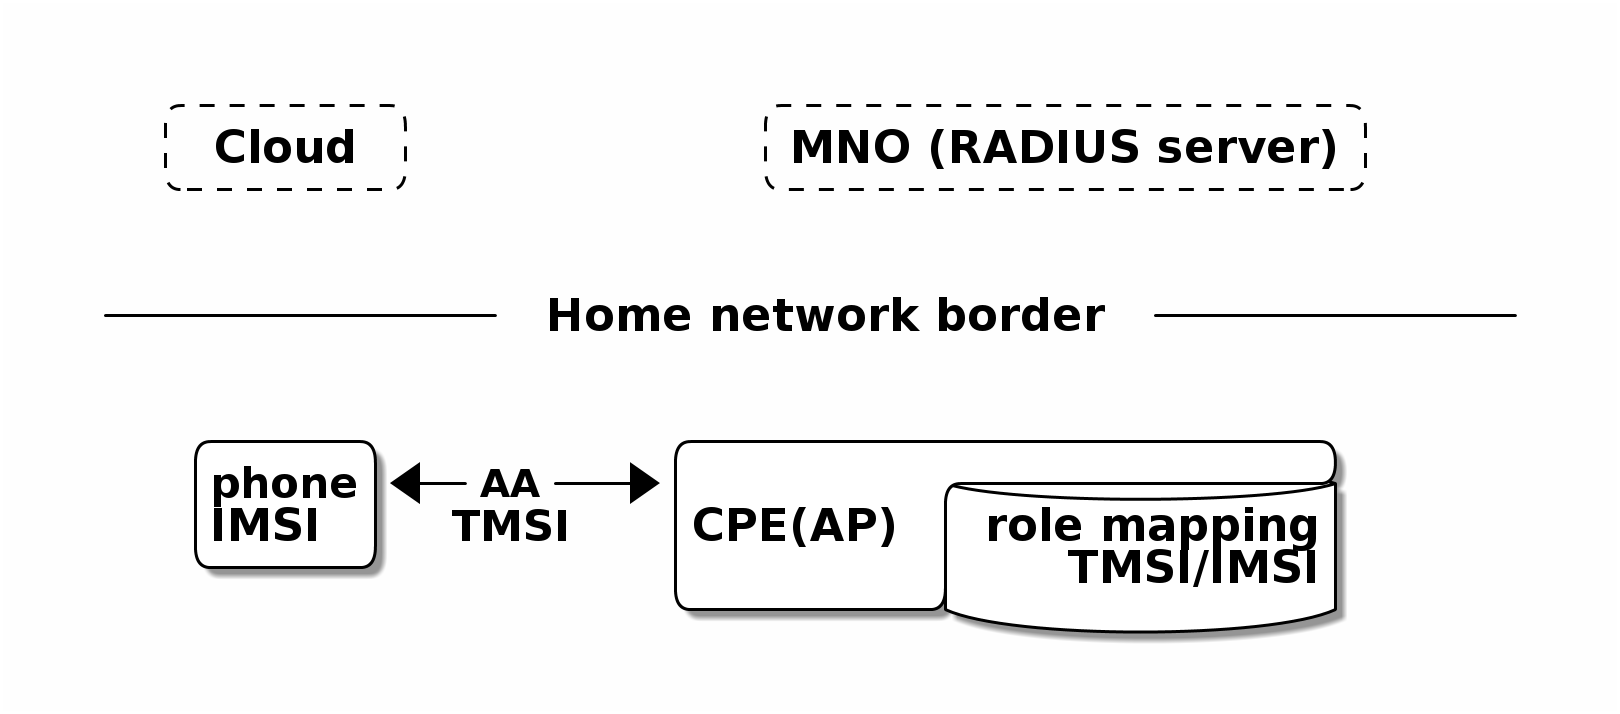
\includegraphics[width=.9\linewidth]{scenIV.png}
\caption{\label{fig:scenario-IV}Scenario IV, offline}
\end{figure}




[repeat the same, To be combined]
The local CPE may cache AuthZ information. It also 
saves the session information and next possible TMSI values. 
When the smart phone makes a re-authentication request with
its temporal IMSI value, the CPE still would know the connection to 
the right mapping to IMSI authorization.





In case that nothing has been configured in network, there are no 
admin users and APs are set to factory default, then they need
pre-configuring and bootstrapping. The scenario can be any of I-IV,
but CPE has neither trust nor roles. Bootstrapping is discussed in 
Section \ref{bootstrapping}.


\section{Modification of RADIUS messages [perhaps to security integrity chapter?]}
\label{sec-4-3}
\label{sec:radius-macs}

Our model would greatly benefit from the modification of RADIUS messages in proxying
RADIUS, if that is possible as was mentioned in Section \ref{sec:radius}(RADIUS).
The modification is needed, when the proxying RADIUS wants to combine AuthN message
from MNO to AuthZ decision received from elsewhere.




RADIUS messages are normally not protected from eavesdropping, but they have
integrity fields to notice if tampering has been done. 
Integrity field is called a Message Authenticator.
Notice the use of the term \emph{Authenticator} in different context here, not
meaning 802.1X's Authenticator.
When using RADIUS to AuthN and AuthZ, Requests can only belong to ACCESS-REQUEST messages while
Responses can be any of ACCESS-ACCEPT, ACCESS-REJECT, or ACCESS-CHALLENGE message.
The Message Authenticator field is sent as last Attribute Value Pair (AVP)
of each RADIUS message and it can belong 
to either Request or Response.\cite[p.20]{radiusbook}.

The Request Authenticator is 16 octet long, random number in
ACCESS-REQUEST message but the Response Authenticator for it is achieved
by one-way MD5 digestion function. 
The digest is taken from concatenation of Code, ID, Length, corresponding
Request\-Auth, Attributes, and a Secret and can look like 
$3fef65608\ldots 2a79$. 
\begin{verbatim}
 Response Authenticator = 
     MD5(Code |ID |Length |Request Authenticator |Attributes |Secret)
\end{verbatim}
The Secret is the shared secret which has been configured between
RADIUS client-server pairs,
and it protects some parts of traffic. 
Different RADIUS client-server pairs may use different
shared secrets and RADIUS server must separate them by client's IP address to
manage proxied RADIUS requests\cite{radiusbook}.

An exception to above mentioned plain-text messaging are the user passwords.
If the user password was to be transmitted in RADIUS, it would be sent first
through exclusive OR (XOR) function together with MD5 digested Secret
and Request Authenticator.
\begin{center}
{\tt 
User-Password = XOR(password, MD5(Secret | Request Authenticator))}
\end{center}








RADIUS servers may implement different vocabulary in their AVP set.
RFC6929\cite{rfc6929} reminds, that even when
the RADIUS proxies do not understand all AVPs inside RADIUS message, they
must deliver those attributes and that allows us to use larger set of AVPs 
than is in any (proxying) RADIUS server's vocabulary.
By adding AVPs inside the authorization packet, we achieve extra
information about validity of the access request.
That information may include a VLAN parameter or a timestamp for a forced
logout.
RFC2865\cite{rfc2865} says, that the forwarding RADIUS proxy may alter
the packet as it passes it, but because an alteration would invalidate the
packet's signature, the proxy has to re-sign the packet.




So at least Proxying RADIUS can insert something, but that is not
enough.  If a malicious actor imitates RADIUS Proxy (i.e. Man in the
middle, MiTM), it can try to inject false messages. 
The Message Authenticator with MD5 digesting
might help in detecting those attacks,
Unfortunately MD5 can not be thought computationally
secure, because duplicate hashes are easy to compute
today\cite{xie2013fast}.
MD5 hashes were first time broken by brute force
already 20 years ago and today they can only be used as a data error
detection tool\cite[p.2]{rfc6151}. 



\section{Similarities with Lock-and-Key method}
\label{sec-4-4}
The method is very similar to the concept used on routers to dynamically enable
access to certain parts of network by first letting the user to log in
to the router. If the access succeeds, the router dynamically adds
route to the management (or other restricted) part from the 
users network.









\begin{figure}[htb]
\centering
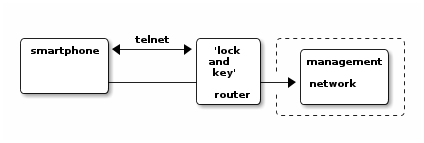
\includegraphics[width=.9\linewidth]{lockandkey.png}
\caption{\label{fig:lock-and-view}Cisco's view of Lock-and-key access}
\end{figure}




Device provider Cisco calls this
 ``Lock-and-Key''
access and uses dynamic access list to implement it\cite[p.117]{lockandkeybook}.
Lock-and-key is presented on Figure\ref{fig:lock-and-view}.
 Smartphone has only limited access to the network before AA
has completed, while in the Lock-and-key
the other parts of network are already open and successful login to the router opens
access to even more segments through it. In other words, Lock-and-Key
protects IP-access in layer-3 and though needs IP addressing, while
802.1x's protection starts already at layer-2 between the smart phone
and AP. Captive portals are similar to Lock-And-Key.


Both methods, 802.1X and Lock-and-Key (and captive portals) can have RADIUS as an Authentication server. 
When RADIUS is not available, for example because internet is down,
there almost always exist as a failover a local password method in the configurable 
router.




[This belongs to multiple SSID section]

If Lock-and-key method was used instead of EAP-SIM RADIUS, then
separate manage\-ment LAN would not be needed. Roles were given at
Authentication server or designated router after the smartphone has done login to it
via normal access network.



This thesis suggests a mix of these methods: EAP-SIM 802.1x WPA2 for
authenticating and encrypting in the local network with SIM and
Lock-and-key type modification in the AP to further access the 
management network. Finally, RADIUS protocol is used to transfer 
parameters, that the smartphone would need in communicating with 
devices in need of changes.

\begin{figure}[htb]
\centering
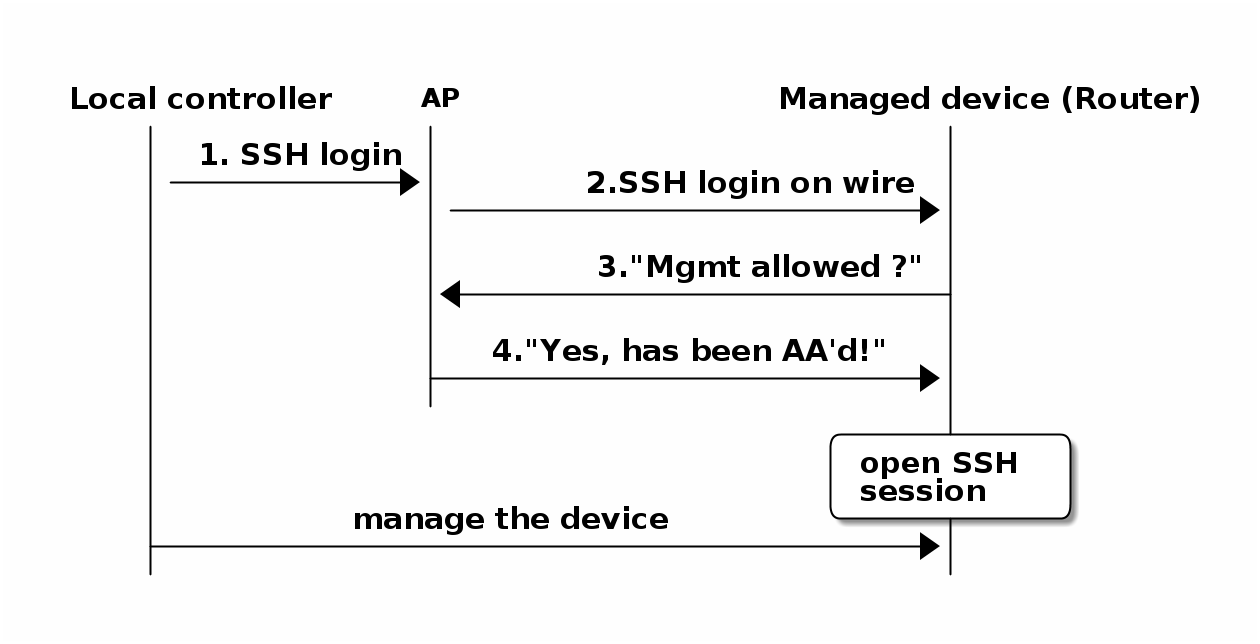
\includegraphics[width=.9\linewidth]{trust-register.png}
\caption{\label{fig:trust-register}trust register (draft)}
\end{figure}

\begin{itemize}
\item register itself to registrar or function as registrar itself!
\item software for that
\end{itemize}




\begin{enumerate}
\item Smartphone connects a Router via wireless AP, and needs to login
\item Smartphone uses telnet (or ssh) to login to the ROUTER.
( but with which credentials?)
\item ROUTER(as RADIUS client) checks AA from Authentication Server(or 
proxy)
\item AA-server answers based on earlier SIM-authentication that this
request is correct
\end{enumerate}



\section{Chosen management model}
\label{sec-4-5}





The simple way to propagate changes from the cloud (or any outside
source) is to make them come from the trusted place, here the smartphone,
where an application takes care of sending them right to the end
devices. This simplification has some pitfalls. If the smartphone continuosly stays
in the management network, then the changes coming later may not be 
separated from the currently approved.
If we understood that the change approval belongs to the AA-process, then
the later approvals would also need an AA.

 The smartphone should either be dropped out from the management
network right away after the changes have been sent or after a
predefined timeout period during which more changes can be send.
That period can be called a management session.
The session time and the logout can be handled in AP directly with
an timer. After a specific time AP simple drops the connection
(WPA2-session) to the phone. This needs modification to the AP
software, if there is not already such method.

Other solution would be for AP to listen for a command from an external
AuthZ server, where similar timer would trigger a notification event. 
That also needed modifications;  a listening process to the AP and 
the timer into the AuthZ server. 
If GBA architecture was chosen, then the smartphone would hold a 
token with a validity time and has to present that when accessing
services, here the management network. 


To demonstrate how the model works, we present the case of adding a
new admin user. Let's first suppose, for case of simplicity, that the
home network has been already configured(bootstrapped) and it is
functioning properly.  The home configuration model has been copied to
the cloud.  When changes are made to the cloud model through
authorized cloud administrator users (operators), those changes are
later also committed in to the production in home network. There is no
magic here, plain configuration change, just this time externally
initiated.

Now, let's think what happens, when the cloud operator (or owner of
home network) tries to modify attributes, which give access to a new actor,
such as a new operator, who would want to have access to separate
segments of home network.  First we need to have that segment separation
change approved and after that we want to allow the newcomer account
to have access to that segment and only to that. For the first part,
which is normal operation, approving would perhaps yet not be
necessary, but for the second part we need some checking unless our
trust to cloud operator is ultimate.  

When CPE of home network is about to input configuration changes which
would change the balance of authors or roles, it needs to check that
the change is permitted.  Permission needs to be asked from a trusted
point, here mobile SIM. Instead of that, the CPE checks from its own
state database, whether mobile SIM has been given access to management
network.
This thesis justifies the management and therefore the changes to be
allowed, if the smartphone user is currently logged in to the
management network.


It must be noted, that the smartphone can already have an association
to a non-management network with Wi-Fi. If that is the case, it first
must disconnect from there and then connect, i.e., do the  AA in the correct management
network. This implies disconnection from other services using Wi-Fi
link, because smartphones currently have only one Wi-Fi radio
available and routing would still prefer Wi-Fi as a default gateway, although
possible 3G data link still may stay up and operational.

\section{Summary of the chosen solution}
\label{sec-4-6}

[wrap up of solution]

The chosen solution to benefit from SIM is via EAP-profiles, as EAP
is well known when using WPA2-Enterprise protection in Wi-Fi.

Design is [move from above]\ldots{}
and it is a variation of lock-and-key design.

Above it was mentioned, that the local controller delivers changes to each
device. 
On this work, it is first assumed that the local controller (smart
phone) only \emph{approves} changes,
and delivers them to \emph{one, central CPE}, 
which handles distribution of changes to other CPEs. The distribution
is not further described. 
Later, the Authenticator is both the AP and
RADIUS client (in scenarios I-V), which receives RADIUS messages from
Authentication server, even when there would be a separate local RADIUS server
running as a proxy.
Lastly, a variation of the design is, that not every change needs to go
 through  the local controller and so the process does not always need
interaction from the user. For example, if 3rd party has been given 
a right to switch on and off its sensor network, it would not be 
necessary for the home owner to accept those changes every time they occur.



Critical changes are those, where network topology changes so much,
that different players would get access outside their earlier domains.
Different players include external service providers, users at home,
visitors, and also home network owner. Examples of the previous cases can first be
seen on the division of home network to guest and private network and
extensions for homeworkers instead of office.



\chapter{Implemented Solution}
\label{sec-5}


To prove that the proposed model works, empirical tests were done.
A preliminary plan to benefit from SIM-authentication at home is
presented in Figure\ref{fig:sim-pre}. The real operator (MNO) and its HLR were 
planned to be replaced with a gateway at home network and the real phone
with its simulated counterpart. HSS would replace HLR in 3G/UMTS
networks. 
Only the Local Controller's interaction with the home network is
tested and Cloud part set away.

\begin{figure}[htb]
\centering
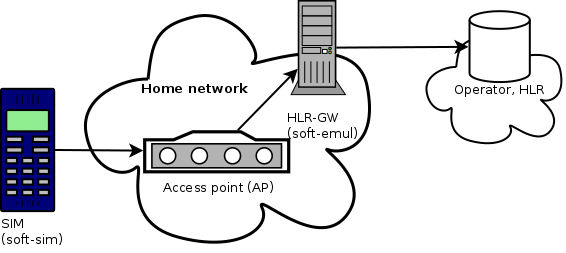
\includegraphics[width=.9\linewidth]{phone-soft-hlr.png}
\caption{\label{fig:sim-pre}Plan to benefit from SIM-authentication at home}
\end{figure}

First it is shown how EAP-SIM authentication works in a simulated
environment.
 Then a use case for disconnection is reported and network traces are analyzed.
In the end, it is shown, that the changes in the management network are possible from
the local controller with  command line interface (CLI).



\section{EAP-SIM authentication test bed}
\label{sec-5-1}



Physical devices used in the tests  were three smartphones, an Wi-Fi accesspoint, and a laptop.
The smartphones were Nokia E70-1, Nokia E90, and Jolla. The Nokia phones
featured EAP-SIM by factory, but the Jolla phone missed a crucial
software library
and right compilation time configuration set on its WPA-supplicant for SIM.

Jouni Malinen's software package \emph{HostAP}\cite{hostapd} provides
components for WPA2-Supplicant, Wireless Access point (AP),
HLR-gateway (for GSM networks), and EAP-endpoint with or without
RADIUS-server. From those, wpa-supplicant, hostapd for wired RADIUS
server, and hlr\_auc\_gw programs were used.  
The versions of \emph{HostAP} used in the tests were 2.2 and later 2.3,
while version 2.4 was published on March 2015 and 2.5 on September 2015. The software
may be distributed, used, and modified under the terms of BSD license.

For a more realistic test, additional hardware AP running OpenWRT
firmware was used instead of hostapd's AP. OpenWRT AP worked as a
RADIUS client connecting to the RADIUS server still provided by the
hostapd.  OpenWRT AP did not try to open EAP-messages, but just
encapsulated them into RADIUS packets.  RADIUS server's configuration
file can be seen in Appendix \ref{app:radius-conf}.


Laptop's role was therefore physically split-brain; it asked for AA in
the end from itself.
Figure\ref{eap-sim-testbed} shows how EAP-SIM AuthN messages (dashed
and solid arrowed lines) flow when using 
simulated WPA2-Supplicant and HLR-AuC as simulation environment.

To make thing more interesting, laptop's WPA2-supplicant with know
software SIM part was later implemented inside Jolla. This was
possible thanks open software and similarity of Jolla's environment to
used in laptop. Modification involved compiling PCSC-libraries and
recompiling the WPA-supplicant used in Jolla with simulator options 
for ARMv7 architecture.



\begin{figure}[htb]
\centering
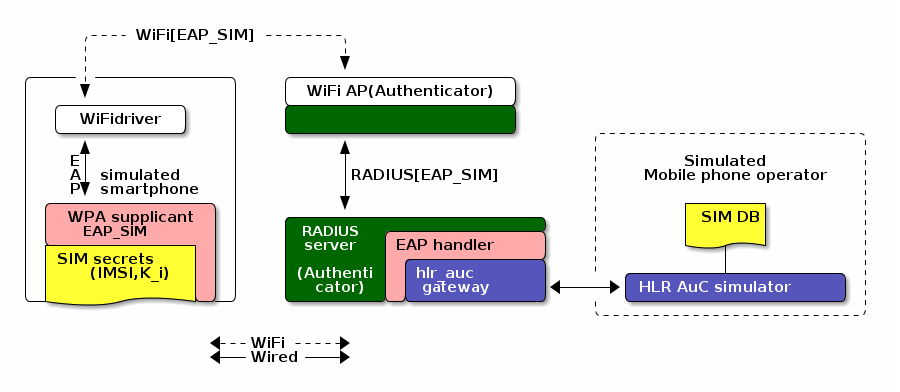
\includegraphics[width=.9\linewidth]{demoinfra.png}
\caption{\label{eap-sim-testbed}EAP-SIM AuthN messaging in simulation testbed}
\end{figure}





The algorithm used in the demo was an internal GSM-Milenage,
which handles EAP-SIM beside EAP-AKA.
Milenage is a reference implementation and as such suitable for operators, who do not 
want to invent their own security algorithms. OPc and Seq parameters from
Milenage were not used, because they are not needed in EAP-SIM. 

\section{Detailed description of test runs}
\label{sec-5-2}





The first tests were done with hostapd as a wireless AP.
Test run with Nokia E70-1 with Symbian 60 Series OS (2006) had a
non-registered SIM card. Despite that it took part in generating
primary EAP traffic. 
Examples in appendix \ref{app:nosim}   [TBD]


Nokia E90, with a registered SIM had better results. Traces
are in folder \verb~gitdocs/di/testit/~ files \verb~eap3.pcapng~,
  \verb~e90.sim.auth.pcapng~ and \verb~eap-1.pcapng~  [TBD]



After some modifications, runs got to the authentication phase.
Naturally, challenge-responses did not work because SIM secrets were
not known. Nevertheless, both cards succeeded to the point, where MNO's
message would had next been verified with the SIM card.

Unregistered SIM in phone could not use SIM card at all, while 
phone with a registered SIM verified and noticed, that operator is not right, 
and therefore correctly ended the conversation as it should regarding
RFC4186\texttt{rfc4186}.

At this point, physical phones were put aside and a simulated SIM-card
environment was used.
After WPA2-Supplicant run on laptop with simulated SIM-card access 
with SIM/USIM protocols, respective EAP-SIM, logging 
from hostapd software claimed that 
\begin{verse}
"Hostapd will send SIM/AKA authentication queries over a UNIX domain \\
socket to an external hlr\_auc\_gw program." \\
\end{verse}
Appendix \ref{app:hlraucgw}   shows that traffic.

Tests were run from a shell program (Appendix \ref{app:fulleap}), which
started the needed programs. That also recorded used configurations, logs,
and traffic captures for later analysis.


\section{Disconnecting the local controller and offline changes}
\label{sec-5-3}
\label{sec:disconnections}
[Limiting time and forced logout, for how long access provided to
management operations, or use fast-auth on following accesses TBD]

After the phone has been successfully connected to the management network,
changes coming from 
the phone can reach routers.  There should be a way to close the session after
the changes has been applied. Originally it was thought, that the session
would stay open only for a limited time, after which the phone would be forced to
logout or thrown away from the management network and that idea should be
kept in mind when the final implementation is made.





Later it was learned, that terminating a session is not included in the original RADIUS protocol.
The root cause is, that messages originating from the RADIUS server
are not defined in the RADIUS protocol and so AP as RADIUS client cannot
receive RADIUS server initiated disconnection messages. 
Additional
extensions such as Disconnect and Change-of-Authorization (CoA)
packets, also known as RADIUS Dynamic Authorization or RADIUS
Disconnection Message(DM), have later been brought in\cite{rfc5176}
to the protocol by diverse vendors, but they may not all be implemented on
every device.
Disconnect-Request is sent to UDP port 3799, so Authenticator should
listen also that in addition to RADIUS UDP port 1812.
As a side note, Diameter protocol would provide server initiated messaging.












[ Back in track: this can be left here ]

\begin{itemize}
\item forced logout, like in captive portals, where RADIUS is not used.
\item no straightforward solution exists within RADIUS
portal [-> reference to \hyperref[text:nointernet]{No Internet connectivity} link is
\end{itemize}




To defeat internet connection problem, a simple solution would be
sending a one-time password to a predefined phone via an SMS, but what
entity would then check that and who would be authorized to send that message?
Authenticating server, which has no internet connection should 
have a predefined way to check that one-time password received via SMS is correct.

Solution for this could be still using a co-existing captive-portal
for emergency access. As AP is programmable with luci, it could
provide this portal.  Alternatively, existing programs such as
\emph{ChilliSpot} or \emph{NoCatAuth} could be used as WWW-portals.  For that to
success, the WWW-portal would also need an open access without 802.1X
port based access control.


\section{Network traces (EAP, SIM, AUTH traffic analysis)}
\label{sec-5-4}
Wireless capture of traffic between WPA2-Supplicant and AP was made at
WPA2-Supplicant on the wireless card. Capture was
not made in monitoring mode, so not all 802.11 details in
data packets were captured\cite{wireshark-capture}.
That was not a problem, because the focus was 
in the EAP messaging instead of radio channel details.
Whole conversation is given first here and afterwards analyzed more
thoroughly.

[TBD: normalization of frame numbers (change ids and timeformat). Capture points in picture.]




First capture shows tries with normal phones, when SIM secrets were
not known. Even when authentication conversation would not complete fully,
Authenticator still received a claim of identification from the
smartphone. Yet, as there is no AuthN, no proof of identity existed in
that case.

[Missing trace, demonstrating the use of unknown SIM physical phone,
include first traces: TBD.]  


Packet capture of successful SIM-authentication with corresponding
parts of logs at WPA2-Supplicant, RADIUS server and packet captures
802.1X, RADIUS and HLR is shown below.  Communicating partners are
denoted as AP-802.1x and smartphone for Wi-Fi traffic, AP-wired and
RADIUS-srv for RADIUS on wire, and finally RADIUS-hlr and HLR-AuC gw
for simulated MAPS/SS7 traffic.
The capture has been done at the WPA2-supplicants end.


\scriptsize
\begin{center}
\begin{tabular}{rrlllrl}
No. & Time & Src & Dest & Proto & Len & Info\\
129 & 15:57:17.9830 & AP-802.1x & smartphone & EAP & 23 & Request, Identity\\
130 & 15:57:17.9832 & smartphone & AP-802.1x & EAP & 39 & Response, Identity\\
131 & 15:57:17.9887 & AP-wired & RADIUS-srv & RADIUS & 235 & Access-Request(1) (id=162, l=193)\\
132 & 15:57:17.9889 & RADIUS-srv & AP-wired & RADIUS & 108 & Access-Challenge(11) (id=162, l=66)\\
133 & 15:57:17.9908 & AP-802.1x & smartphone & EAP & 38 & Request, GSM Subscriber Identity\\
 &  &  &  &  &  & Modules EAP (EAP-SIM)\\
134 & 15:57:17.9924 & smartphone & AP-802.1x & EAP & 70 & Response, GSM Subscriber Identity\\
 &  &  &  &  &  & Modules EAP (EAP-SIM)\\
135 & 15:57:17.9945 & AP-wired & RADIUS-srv & RADIUS & 272 & Access-Request(1) (id=163, l=230)\\
 &  & RADIUS-hlr & HLR-AuC gw & socket &  & SIM-REQ-AUTH <IMSI> 3\\
 &  & HLR-AuC gw & RADIUS-hlr & socket &  & SIM-RESP-AUTH <IMSI>, 3 triplets\\
136 & 15:57:18.0024 & RADIUS-srv & AP-wired & RADIUS & 256 & Access-Challenge(11) (id=163, l=214)\\
137 & 15:57:18.0040 & AP-802.1x & smartphone & EAP & 186 & Request, GSM Subscriber Identity\\
 &  &  &  &  &  & Modules EAP (EAP-SIM)\\
138 & 15:57:18.0043 & smartphone & AP-802.1x & EAP & 46 & Response, GSM Subscriber Identity\\
 &  &  &  &  &  & Modules EAP (EAP-SIM)\\
139 & 15:57:18.0063 & AP-wired & RADIUS-srv & RADIUS & 248 & Access-Request(1) (id=164, l=206)\\
140 & 15:57:18.0065 & RADIUS-srv & AP-wired & RADIUS & 202 & Access-Accept(2) (id=164, l=160)\\
141 & 15:57:18.0110 & AP-802.1x & smartphone & EAP & 22 & \em{Success}\\
142 & 15:57:18.0112 & AP-802.1x & smartphone & EAPOL & 135 & Key (Message 1 of 4)\\
143 & 15:57:18.0123 & smartphone & AP-802.1x & EAPOL & 135 & Key (Message 2 of 4)\\
144 & 15:57:18.0161 & AP-802.1x & smartphone & EAPOL & 169 & Key (Message 3 of 4)\\
145 & 15:57:18.0163 & smartphone & AP-802.1x & EAPOL & 113 & Key (Message 4 of 4)\\
\end{tabular}
\end{center}
\normalsize




IMSI is sent first time already on the second EAP message from 
WPA2-Supplicant to AP (compare with Figure\ref{fig:eap-sim-radius}, message 2.)
This part is presented in Capture \ref{capimsi}.

\lstset{basicstyle=\ttfamily\small,
  columns=fixed,emph={1232010000000000}, 
  emphstyle={\color{red}\textbf}}
\renewcommand{\lstlistingname}{Capture}

\begin{lstlisting}[language=bash,
  label=capimsi,
  caption={First indication of IMSI}
]

Frame 129: 15:57:17.983047
    Type: 802.1X Authentication (0x888e)
    Version: 802.1X-2004 (2)
    Type: EAP Packet (0)
    Length: 5
    Extensible Authentication Protocol
        Code: Request (1)
        Id: 50
        Length: 5
        Type: Identity (1)
        Identity: 
Frame 130: 15:57:17.983223
    Type: 802.1X Authentication (0x888e)
    Version: 802.1X-2001 (1)
    Type: EAP Packet (0)
    Length: 21
    Extensible Authentication Protocol
        Code: Response (2)
        Id: 50
        Length: 21
        Type: Identity (1)
        Identity: 1232010000000000
\end{lstlisting}
\normalsize

We notice the difference on 802.1X versions; AP uses version
802.1X-2004 in its request while the WPA2-Supplicant
responses with version 802.1X-2001. Here it does not have any
noticeable effect. 

The last line has the important identity field received from the SIM.
Its length cannot directly be seen, but when EAP message's length (21
octets) is reduced by fixed space needed for Code(1), ID(1),
Lenght(2), and Type(1), it yields 16 octets for the
identity. Therefore the identity is not coded as a 
numeral but instead as a string and that brings more flexibility in
the protocol as the Identity can include alphabets too. It also
minimizes misunderstandings, if context gets lost. 
When we remember, that IMSI can not be be more than 15 octets, the extra prefix '1'
denotes that we are talking about EAP-SIM identity. 





EAP client's identity is transformed at Authenticator
(Figure\ref{fig:eap-layers}, Chapter \ref{sec-2}) from 802.1X's 
EAPOL format  into RADIUS format and
sent to RADIUS server. The captured frame between AP and Radius server is
shown
in Capture \ref{fig:capture}.


\lstset{basicstyle=\ttfamily\scriptsize,columns=fixed,emph={1232010000000000,{=User-Name(1)},Identity},emphstyle=\color{red}\textbf}
\renewcommand{\lstlistingname}{Capture}
\begin{lstlisting}[
  language=Python,
  caption={EAP client's identity transformed},
  label={fig:capture}
]

Frame3: 15:57:17.988616
Radius Protocol
    Code: Access-Request (1)
    Packet identifier: 0xa2 (162)
    Length: 193
    Authenticator: 055ff370b9e793c1e39d375aade8033c
    Attribute Value Pairs
        AVP: l=18 t=User-Name(1): {1232010000000000 }
        AVP: l=7 t=NAS-Identifier(32): musta
        AVP: l=27 t=Called-Station-Id(30): 66-66-B3-8A-68-B3:simtest
        AVP: l=6 t=NAS-Port-Type(61): Wireless-802.11(19)
        AVP: l=6 t=NAS-Port(5): 1
        AVP: l=19 t=Calling-Station-Id(31): 5C-51-4F-E7-FA-F4
        AVP: l=24 t=Connect-Info(77): CONNECT 54Mbps 802.11g
        AVP: l=19 t=Acct-Session-Id(44): 5491885C-00000037
        AVP: l=6 t=Framed-MTU(12): 1400
        AVP: l=23 t=EAP-Message(79) Last Segment[1]
            EAP fragment
            Extensible Authentication Protocol
                Code: Response (2)
                Id: 50
                Length: 21
                Type: Identity (1)
                Identity: 1232010000000000
        AVP: l=18 t=Message-Authenticator(80):04ea7e507d72bdb1acf515ef19ac9527
\end{lstlisting}
\normalsize


Here interesting part is the first RADIUS AVP.
While encapsulated EAP fragment naturally carries the Identity=``1232010000000000''
field, it was surprising that RADIUS has captured that field and 
filled its User-Name field to the very same, ``1232010000000000''. 
IMSI is ``232010000000000'' and it is prefixed with
an '1' as earlier explained.

In WPA2-Supplicant configuration file (see Appendix \ref{app:wpa-conf}) both the identity and
credential section had the identity field, but that might 
just be syntax issue.
AP just has followed conventions on converting
EAP into RADIUS message and put identity field into User-Name
Attribute Value Pair (AVP).
Similar convention can be seen when analyzing EAP encapsulation and
message size. The last RADIUS (AVP) is 
Message-Authenticator, which presents limited safety against message 
corruption. Limited, because it uses MD5-hashing which is not safe
against malicious use anymore.

[Here conversation]



[see. /home/itapuro/gitdocs/di/testit/demot/ap-s150123-155714]

Meanwhile, HLR simulator was listening requests from Authentication
server's internal EAP-handler through a local socket.
The AuthN request (SIM-REQ-AUTH), which in production version would go
to real HLR-AuC, included the IMSI and parameter
"3", which indicates, that the requester wants three triplets. 
While one triplet would equal 64-bit key used for challenges, three
triplets will make the key 192 bit long. [theoretically.. see the
article smwhere].  Format of triplet received is RAND:SRES:Kc.

\scriptsize
\begin{verbatim}
Received: SIM-REQ-AUTH 232010000000000 3
Send: SIM-RESP-AUTH 232010000000000 
 a5dc7c1a177ee418:fea4260f:6634b5081c74b5872b49f37fc387ddb5 \
 0faa08f223510ef6:e6d0f3f4:3d7559287e5bd2ec3fb77b1f7d097d8f \
 832475ad3e7bea2b:3fe28cc8:1be8b4f1ab247ec732d15cf63ad57390 \
\end{verbatim}
\normalsize

\section{Simulation on smartphone Jolla}
\label{sec-5-5}

Because we had source code available, we also tried to move 
the simulated SIM application to the real smartphone.
Jolla is a finnish smartphone, running on ARMv7 processor, having its
root's on Nokia's last mobilephone operating system MEEGO.
The OS is called Sailfish and it includes user interface code made by
Jolla, open source components from Mer (MEego Reinvented, or
meritocratic community), and some 
other software components, which are either free or proprietary.
Jolla's base 
WPA-supplicant belongs to Mer core and it was here re-built for 
simulator use. The build process was done inside the Virtualbox
program, because it provides simulated Jolla environment and
 made porting programs to Armv7 processor easy.


\begin{center}
\begin{tabular}{rll}
version(s) & component & tested on\\
2.3 & hostap(RADIUS-EAP) & laptop(x86\_64)\\
2.3 & hlr\_auc\_gw & laptop(x86\_64)\\
2.2, 2.3 & wpa-supplicant & laptop(x86\_64)\\
2.4 & wpa-supplicant & Jolla (armv7l)\\
1.1.9.28 & Sailfish & Jolla (armv7l)\\
1.1.9.28 & Sailfish & Virtualbox (x86/armv7l)\\
\end{tabular}
\end{center}



\chapter{Analysis, Results and Discussion}
\label{sec-6}

We have now gone through theory, design and implementation so let's
discuss some results and findings. We concentrate on security, 
deployment difficulties and costs, platform issues and cases where we
need to extend the number of SSID's. The facts collected in the thesis
are once more wrapped up in Discussion section.
Last, we speculate on some alternative design solutions for adding
trust and management models.


\section{Security considerations}
\label{sec-6-1}



There can be multiple ways to attack the described methods of
the home network management delegation. Following subsections divide them into
confidentiality (privacy), integrity, and
authenticity. Accessibility is also discussed.
\subsection{Confidentiality (privacy)}
\label{sec-6-1-1}

The purpose of the message confidentiality in authentication phase is
to hide the identity of the smartphone and possible the delivered
secrets from eavesdroppers. Hiding IMSI enhances the privacy of the smartphone user. 


Recall from Section \ref{sec:sim-based-auth}, that IMSI is sent in clear 
during the starting phase of 802.1X authentication and that is a privacy 
issue, because TMSI which hides IMSI cannot be used before a session
has been set up.\cite[p.66]{rfc4186}.
After the first full authentication, the client and the Authenticator 
know TMSI and can use it in further communication. 
TMSI can even be re-changed using re-authentication as shown in Figure\ref{fig:tmsi}.

\begin{figure}[htb]
\centering
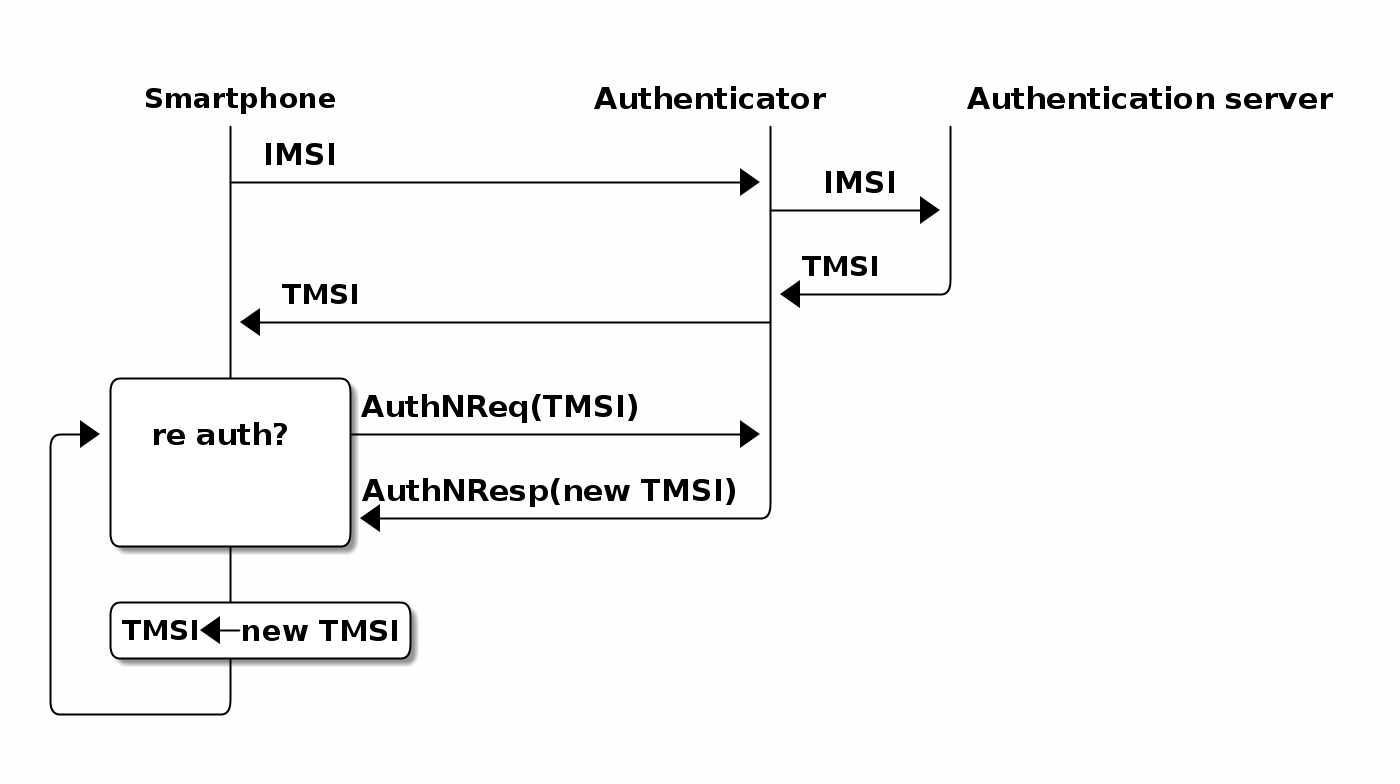
\includegraphics[width=.9\linewidth]{imsi-tmsi.png}
\caption{\label{fig:tmsi}Changing TMSI without MNO or Authentication server}
\end{figure}




The Authenticator 
is responsible for converting  TMSI to IMSI if it later needs to 
ask for full authentication from the MNO. During that time,
IMSI can be caught using the device called IMSI-catcher.

The very same happens also in a regular GSM network with non-EAP traffic.
IMSI can be caught by listening the GSM network for phones that are
registering themselves to the operator when they are powering on.
The fault lies there, that GSM specification does not require the
mobile network to authenticate itself to the phone and so GSM allows
man in the middle attack. 
The attack follows, when the IMSI-catcher impersonates itself as a
(cellular) base station.  When the smartphone tries to attach to the fake base
station, the smartphone reveals its IMSI number. Further, because the
base station is responsible for chosen encryption, the base station
can order the phone to not encrypt traffic at all or to use only weak
encryption thus revealing all data, calls, and texts. Mitigation for
IMSI-catching would be to disable GSM (2G) usage altogether from phone
if that is possible\cite{imsi-heise}. Some development has been done to detect 
IMSI-catchers, most notably by the project AIMSICD\cite{aimcid}.


Most EAP methods do not provide identity protection, i.e., the
end-user hiding themselves.
This can be achieved with PEAP (Protected EAP) or TTLS, which
chains different EAP-methods together and protects the inner EAP with
an outer EAP. 
The outer identity tells just the realm, where AuthN can be checked
and inner identity reveals the real identity.  The inner identity is
encapsulated inside the outer identity which functions as an
envelope. 
For example EAP-MSCHAPv2 (Microsoft's Challenge
Handshake Authentication Protocol, version 2) can be used inside PEAP.


EAP-SIM would provide identity protection, if it was used together
with PEAP which protects the outer identification  and
then EAP-SIM was used in inner authentication.
Currently it is not known for the author that such implementations exists for
EAP-SIM  except Tseng's proposition\cite{tseng-usim} for a new EAP type
EAP-USIM, which would extend EAP-TLS type.

If it was possible to use anonymous identity on outer EAP
authentication, then EAP-SIM AuthZ must also be done at HLR AuC.
AuthZ cannot else be connected to the corresponding
identity and AuthN itself is not enough because it only defines the users'
authenticity, not their admin roles and so 
AuthN should work for any  smartphone that has existing contract with
their MNO. 
It still is the responsibility of the Authenticator to 
check AuthZ  and let only admin mobile access the management network.

If SIM is used as the only EAP without EAP-PEAP, then there is no
mitigation for revealing the IMSI on the first message and it leads to
privacy issue.  If there was an IMSI-catcher involved, only IMSI would
be revealed.  The other parameters or encryption are not in danger in
EAP-SIM authentication, because EAP-SIM will stop conversation, if it
does not receive the correct MNO authentication message.  EAP-SIM
protocol, as do most of the other EAP-variants, provides a secure way
to generate session parameters to WPA2-session and those are not
leaked outside, because they are created individually on both
endpoints: at the smartphone and at the Authentication Server.
Finally, the fact that the secret key Ki stays inside the SIM makes it
difficult to attack the session by pretending to be the smartphone.






RADIUS messaging is vulnerable too, because it includes IMSI in clear form 
inside EAP encapsulation. IMSI is also included in a RADIUS user-name
attribute includes also IMSI, because it has been transferred there from
from EAP's identity field.
RADIUS runs over UDP, but can be used also with TCP with the RadSec
extension. RADIUS servers usually support that extension, but APs do not, so 
there will be parts, where RADIUS messages travel in plain.




Based on those facts, EAP-SIM cannot be considered confidential for identity
during first message exchanges, but later the identity can be hidden
using temporal identity (TMSI). 
For other parameters, EAP-SIM is confidential.
Thus, this paper does not consider TMSI in the implementation Chapter
\ref{sec-5}.
\subsection{Integrity}
\label{sec-6-1-2}



The integrity issues were handled in Section \ref{sec:radius-macs} describing
RADIUS message modification.
Message digestion codes provide integrity for RADIUS protocol.
If PEAP is used, it handles integrity through its usage of
 TLS\cite{peap}.
Above mentioned RadSec extension allows other digesting functions than MD5 such
as SHA1 and is open for negotiating more secure ciphersuites that later
versions of TLS might in the future require\cite{rfc6614}. This is
even more important, as it already has been noted in 2005, that SHA1 can be
broken

There is also a fraudulent Authenticator problem, which is an attack
against both the integrity and privacy.  The Authenticator may present
some information to the Authentication server and other to the
EAP-peer. Mitigation for that is, that EAP-peer includes some
characteristics of the Authenticator inside its EAP-message, which
the Authentication server then verifies (RFC6677)\cite{rfc6677}.

\subsection{Accessibility, DoS and Scalability}
\label{sec-6-1-3}

Is home network immune against (distributed) denial of service (DoS)
attacks? Besides DoS, does the solution scale up from home network to
small and middle size companies?
To answer this we can remember that backends (cloud and operator) are
designed for thousands or even millions of users, so 
they hardly are limiting factors. Instead, local
Authenticator is the one whose performance might suffer, which
comes from processing loads\cite{2009-lin-simefficiency}.


Traditionally, RADIUS has used connection\-less UDP protocol that is
light weight. UDP misses reliability that TCP has, and retransmission in UDP is
tolerable, because the user is ready to wait  several seconds for
authentication to complete. Today, RADIUS can also run over TCP, which
has generally more aggressive retransmission
rate\cite[Section 2.2.1]{rfc5080}. 
On the other hand, adding an
alternative UDP RADIUS server can answer faster than waiting for TCP's reliable delivery.


\subsection{RADIUS weaknesses and strengths in limited use cases}
\label{sec-6-1-4}


RADIUS protocol itself is old and not very secure as of current
standards(2015), because messages are not encrypted and they are
transported on datagrams (UDP). Alternative RADSEC protocol uses TLS, and 
is backwards compatible with RADIUS protocol, so it can be used
as secure RADIUS proxy such as \emph{radproxy}\cite{uninett-radproxy}.

RADIUS uses MD5 hashing and shared secrets. Because of the weaknesses of
MD5 hashing (for example MD5Attack\cite{rfc5176}), the transport needs additional
protection like tunneling or IPsec. TLS can be used for encryption and
its signatures for integrity checking of packet payload.
RADIUS protocol itself provides some integrity checks with Message
Authenticators as described in Section \ref{sec:radius-macs}.



In scenario III(Figure\ref{fig:scenario-III}),  there was a proxying RADIUS between Authenticator
and MNO.  When MNO notifies Authenticator
that a smartphone has been authenticated, then Authenticator (AP, functioning
as a RADIUS-client) hooks that message and usually just grants
smartphone the access to the network. After giving access rights, other
provisioning parameters can be sent with RADIUS messages, for example
session time-out,
current admin user list, state of OTP list, or VLAN id.


\subsection{Replay, Re-use, Re-auth, and brute-force challenges}
\label{sec-6-1-5}

Earlier in RADIUS analysis, prevention of replied messages was
mentioned. Reusing the same secret in different security context is also
considered bad because mixing secrets between usage
domains weakens the security.  In GSM networks, IMSI identifies subscriber on
first contact, later TMSI is used for call and SMS.  In EAP-SIM those
values are also used. IMSI naturally is the same, but TMSI should be
different for call and EAP.  Haverinen\cite{hav-doc} explains how
special RAND numbers can be used to differentiate the use of TMSI in 3GPP and LAN
contexts.

Re-authentication and termination can bring unexpected results.
If SSID changing introduced in mitigation Section(\ref{tag:hidessid}) was in use, fast re-authentication
should be forbidden\cite[p.11]{rfc5448}.
Even, when sessions can be terminated, the client side may have 
option set to login automatically, transparent and without users control.
Automatic re-authentication after disconnection  must be considered
here as harmful as well as automatic login when nearby suitable AP. An
example from harmful behaviour is Swiss mobile operator Swisscom, who
 provided two networks ``Mobile'' and ``Mobile Eapsim''  for its
customers. 
The latter network did not ask customers
for connection but used theirs smartphones' SIM automatically. Unfortunately,
it also charged users for using Wi-Fi connections without users'
knowledge.\cite{swisscom}



If one can read and write data through SIM card's API,
one could try to get information (SRES, Kc) by brute-force. 
Fortunately SRES and Kc are never sent in clear, but inside
a digested MAC.
 Additionally SIM card can be programmed to answer only
limited number of challenge request, for example 65535, which in
normal usage would be enough, but in brute-force challenges 
it would soon be exhausted and not function anymore.


\subsection{Hardware tampering}
\label{sec-6-1-6}
All this time it is assumed, that hardware does not lie. In case
the hardware has been tampered, we could not trust it and its claims.
For example, there have been attacks against SIM to reveal its private
key after SIM have been copied.  To verify, that a device has not been
tampered, a method called attestation can be used.

A device which has attestation capability such as 
hardware certificates or Trusted Platform Module (TPM) technology
can function as a trust anchor.
Such a device could be sent direct to customer with pre-configured
secrets and methods to take a place as a trust anchor. 
That leads us again to the key distribution problem.


\subsection{Mitigation methods against radio capturing}
\label{sec-6-1-7}
To mitigate risks for radio capturing, two methods are presented: hiding of
wireless network and proximity. They are not perfect but can
limit attack vectors in time and place.


Recall that the access to management network from the smartphone is
 needed only then when changes
are challenged. Why then not just enable management radio network
during those times? Then there were less networks for users to choose from.
Enabling management network could be programmed through 
LuCI-interface, which is a web user interface to the Unified
 Configuration Interface used in OpenWRT routers.
Preliminary tests showed, that activating new networks in AP also 
disconnects existing Wi-Fi connections and may even restart AP,
which certainly would not be wanted. Some other methods need to
be invented to avoid denial-of service, when intruder tries to 
connect by that method and causes continuous AP outages.

\label{tag:hidessid}
One could also think of hiding the network by disabling the
advertisement of management network SSID. That is called ``network
cloaking''.  Smartphone would then need to know the exact target SSID name.
Does disabling or hiding the management network bring real security or
is it just security by obscurity?  Security by obscurity means here,
that hiding network 
as a security method would filter out only some casual crackers, while
at the same time it still is trivial for any serious crackers.
Disabling or hiding  merely gives one security layer more so it is not
a real security method.

The SSID could also be renamed always, in essence to implement
one-time-only network, but then the smartphone would need to get that
secret somewhere, perhaps via an SMS and that would defeat the purpose
of easy access.  If that method nevertheless would be used, then
hiding the one-time-only network name actually could add security. 
If the client knows beforehand the name of SSID
(and maybe also checks AP's MAC), then AP does not reveal any information,
before the client has tried to connect to it and that would minimize
the time window for attacks.




 Hiding can also have privacy enhancing effects.
While Wi-Fi client's normal action is to probe for SSIDs of lately visited
and learned APs, analyzing those probes anyone can reveal client's earlier
locations without further effort.
Lindqvist et.al.\cite{hidden-wlan} present usage of hidden
APs in protecting privacy of clients and preventing that scenario.



Regarding boundaries of home network, the Wi-Fi coverage gives 
one natural limit, which is 50 meters indoors or 100 meters outdoors,
when no extenders (i.e. Wi-Fi repeaters) are in use.
Proximity so brings a minimal extra layer just like network cloaking 
for preventing attacks, as the attacker must be physically within those limits.


This can be considered as an added factor in multifactor
authentication or reputation, but it will not be enough, because
attackers will have more sensitive  radios available than normal users
devices have. 
Also, if SIM-profile was used through Bluetooth, there were also
range limits, but even shorter. Despite the claimed distance limits
on Bluetooth, receiving can be extended with even to one mile with
directed antenna\cite{SANS-bluetooth-2007}.




\section{Deployment difficulty and costs}
\label{sec-6-2}

To deploy the system, modifications must be done to AP and client.
Additionally, contract must be made with the MNO service
provider producing AuthN 
For AP, modifications are minimal. Needed settings are
WPA2 mode to WPA2-enterprise, IP-address of RADIUS server providing 
AA, and corresponding shared secret.
For  the client, a Wi-Fi profile must be added: used management SSID,
protection mode 802.1X (or WPA2-Enterprise), and AuthN method EAP-SIM.
Smartphone can have different profiles, also with a same SSID, but
then the user needs to choose manually, which profile is wanted.


While no service yet exists from MNOs, we estimate their costs based
on Mobiilivarmenne. Using Mobiilivarmenne is currently free for
clients, if usage is personal, but costs for service providers are
unknown.  Hardware costs can mostly be eliminated, while users already
have smartphones and for infrastructure, existing hardware such as APs
can be used.

Using SIM to local Wi-Fi AA adds value to the smartphone ecosystem.
To further divide possible costs for EAP-SIM usage
is difficult.
EAP-SIM always needs MNO for first authentication,
because only MNO and SIM-card manufacturer know 
what are SIM's Ki and the used A3/A8 algorithm variation
for GSM/3GPP/LTE authentication.

It is difficult to see if any commercial provider would implement
SIM-key sharing so, that secret part was divided to a part that
implements AuthN for own operator and to a part, that is free to use by
some other operator.  Instead, the same functionality can be achieved with
Dual-SIM phones, which allow inserting two SIM cards from different
operators in to the phone. By using menu option in phone, or even a
specific prefix code before call, alternate SIM card can be chosen
without booting the phone.
Dual-SIM thus allows change of ID and IMSI without removing SIM card.

There exists also private GSM networks. An interesting use case
of them  has been Chaos Computer Club's international 
CCC-camps\cite{ccc}, where organizers 
provide private GSM network for attendees of conference
by distributing them separate SIM cards for 2 euros.  Even, when GSM
network used 1.8GHz radio channel under an experimental spectrum
licence,  GSM encryption also could be used, because the SIM-card secrets were known
to the organizing, private operator.
On the other hand, empty GSM cards for testing can cost as much as 
18 euros a piece (webshop-quote\cite{smartjac-testsim}).


\section{Platform specific issues}
\label{sec-6-3}

For clients, there is no need for public key infrastructure (PKI)
unless EAP-PEAP is used. Under PEAP there are either server
certificate or additionally client certificate present.  There are
smartphones, that do not have EAP-SIM yet available.  For example
support for EAP-SIM (and -AKA) methods starts in Android only from
version 4.x and in iOS from version 5.x.\cite{sim-support}.

Generally, to support EAP-SIM  with open source software in 
smartphone, needed components are \emph{pcsc-lite} for accessing SIM card, \emph{wpa\_supplicant} for
WPA2 client, and possible used connection manager (\emph{connman},
\emph{wicd}, or \emph{Network Manager} in Linux). This is in line, what was done in testing without \emph{pcsc-lite},
because a file backend was used instead of a SIM card.




If OpenWRT platform is used for CPE, the memory size (32MB) restricts
some use.
WPA2 software included in basic OpenWRT installation is small,
but that does not yet include RADIUS server part or EAP-SIM handling.

Software has other limitations. Freeradius2 is not yet included  in OpenWRT.
and if it was, it would also be based heavily on current Perl environment which
itself needs a lot of space.
Currently, as of 9.8.2015, Freeradius is running on version 3 and
EAP-AKA is supported through a module from hostapd project.
COMP128(versions 1, 2, and 3), which is implementation  of A3/A8
algorithms, is  supported\cite{freeradius2}, and so EAP-SIM is available.
Yet, Freeradius can be used as Authentication Center (AuC).
Diameter (freeDiameter) can be compiled in OpenWRT. That is good,
because on 3GPP networks Diameter protocol has more support than RADIUS.
If nothing else works, as a backup old-fashioned WWW-authentication
portal can be used for offline authentication.


\subsection{Access methods to Wi-Fi with only one SSID}
\label{sec-6-3-1}



To enable EAP-SIM method, it is necessary to use WPA2-Enterprise mode
and thus RADIUS server, but at the same time, existing Wi-Fi network at
home usually has been set using WPA2-PSK.
Because it was not found, how Authenticator could use the same network
SSID for both WPA2-PSK (or open access) and WPA2-Enterprise, a
separate SSID for dedicated management network was technically needed.
Luckily, today's APs allow setting of multiple SSIDs.

Nevertheless, if Wi-Fi was limited to only one SSID, then we would
need another 
way to indicate that user wants to get in to management net. 
Separation can be done for example at client's  end by using different realm on
AuthN identity. It also can be done by adding hints for different destination to
username (username decoration) or by using different authentication
method. All these methods allows Authentication Server to distinguish, what the user
wants to do; get normal access to home network or make trust anchor claim to 
management network.


\section{Usability benefits of HS2.0}
\label{sec-6-4}
It is well known, that the usability of the captive-portal Wi-Fi
 network is burden, because a user needs to go through 
a web portal logins with a username-password authentication 
procedure and those are different for every network.
Additionally, the user is often required to switch 
between cellular and  Wi-Fi data access when they change their
 location, and that would disrupt the network connection.

An industry brand  Hotspot 2.0 addresses those issues and tries to
simplify user's switch between Wi-Fi and cellular to automate the
roaming experience.  Hotspot 2.0 is driven by two alliances:
Wi-Fi Alliance has a certification program (Passpoint)
for Hotspot 2.0 compatible devices, while the Wireless Broadband
Alliance has a program called Next Generation Hotspot (NGH), targeted
to user experience\cite{wba-ngh}.

Hotspot 2.0
enables the selection of the network based on the ownership, services and
performance characteristics \emph{before} a Wi-Fi client has been associated
to a Hotspot 2.0 AP. The technology is built on IEEE 802.11u specification. 
In its second release version the operator would
have control on which network the smartphone would carry its data
transmission. 





Ericsson's technology journal ``Review'' revealed in 2012, that their 
HS2.0 goal is ``to make roaming between Wi-Fi and 3GPP/LTE networks smoother
and to bring operator-grade to Wi-Fi by putting control in operators side''. More
than offloading traffic, plans were to bring to Wi-Fi other services too\cite{er-seamless}.
Developing HS2.0 a few steps further would add mobile traffic and internet
off-loading on to Wi-Fi networks and that would be the missing link in
interworking those two worlds.



In Hotspot 2.0, the cellular network may signal the smartphone and
propose it to switch to Wi-Fi. The smartphone then would try to find a HS2.0 capable
access point and continue using Wi-Fi instead of cellular network.
In a similar way, the smartphone could receive signal from the cellular
network, when controlling changes need to be approved. The smartphone
would then make some tests to proof the local AP's suitability for 
HS2.0. If those succeed, then the cellular network would continue and order the 
phone to make a switch to the Wi-Fi network, authenticate there with 
EAP-SIM (or -AKA) and transfer services to Wi-Fi not forgetting 
the transfer in to the management network. This scenario could be 
studied further.


If HS2.0 was used here to automate the part, where
the smartphone needs to change from cellular to local
management Wi-Fi network and back, we probably would
miss the user decision part. The user, not the operator,
 must give his consent to access the management network, so
it is important, that the switch would not be automatic or forced.
In a way, operator aided roaming between Wi-Fi and cellular
works in a different level than here described trust-anchor method.
The operator is interested on the access network, while
we are interested in the side result of getting access, namely 
the achieved trusted access point.






\section{Discussion}
\label{sec-6-5}

Although the core technology has been there for more than ten years and
the hardware and the applications mostly support it, 
there can be many reasons why SIM-based methods are not in wider use. 
One can guess, that the reasons are similar that happened for example with 
WiMax technology, which was used for broadband network connections to
rural areas. Technically that was well enough, but demand was not so
large. Additionally lower speed technologies that were cheaper at that
time, such as cellular modems were thought to be sufficient, even when
inferior technically.
It could also be, that market is waiting for future products, and does 
not want to invest on existing technology, which can be seen as ``old''.



SIM card of the smartphone, used together with Wi-Fi access to home network 
verifies change controls, and for that we have presented some options.

Location of AuthN and AuthZ components may vary depending on state of process.
Always in the beginning, AuthN lies outside the home network, but
later it can use local point. AuthZ, on the otherhand, may be located more freely.

Based on 802.1X standard, the management port is activated and
RADIUS transfers the orders for correct AA.
The smartphone traffic is directed in to an own virtual LAN segment (VLAN),
which is dedicated to the home network devices management.
Thesis thus uses an old, yet simple method for problem risen in a modern environment home network.

Disconnection from a normal (Wi-Fi) access network must happens, before phone can get
into the management network. It means, that all stateful network
connections using Wi-Fi will close at that point. Smartphones do not
have multiple wireless connections, but mobile data connections may 
stay up. Even then, the default routing in the smartphone may change.


EAP does by definition only AuthN part although the successful
authentication often precedes ad hoc AuthZ if nothing else is demanded.
EAP-SIM handles this part, but for AuthZ something else is needed
and so some methods have been presented to add the right role to 
the authenticated identity.



In the design chapter (Chapter \label{cha:design}) it was questioned whether the proxying RADIUS server
can read and alter the messages on their way or is the messaging secured
by encryption, integrity hashes and digital signatures.
Later it was learned, that the message's integrity is indeed protected, if
only in a very light way, but not encrypted.

Altering or addition of  RADIUS messages can be chosen from many
attributes of RADIUS's vocabulary. They can carry extra information
for provisioning in AuthZ phase. Exactly which of them are used
remains to implementer's  decision. 
Term \emph{provisioning} can mean adding users to home network with correct
attributes such as authentication method and identification.
It also can mean identifying users later and giving
them more attributes and access rights dynamically.
Binding a user to a SIM card is also provisioning and that has
happened earlier.













Another problem using in-flight alteration of the AuthZ data in RADIUS ACCESS-ACCEPT message
is the mapping of the authentication messages of IMSI and TMSI identities.
The Authenticator does know the original user and mapping of TMSI to
IMSI, but needs to get AuthZ information. That can be received from the
remote operator, which would be easier for the
Authenticator or there might be a proxying RADIUS, which resolves the AuthZ
information and generates an ACCESS-ACCEPT packet. The latter has issues with
TMSI.

When a proxying RADIUS gets the temporary SIM-identity (TMSI) instead of
a beforehand known IMSI identity, there will be problem
because proxying RADIUS knows for sure only the originating server. 
MNO in turn does not necessary know about the roles.

It seems, that AuthZ data must be mapped during the first phase of
EAP-SIM AuthN, when IMSI still is available, and in some way
that map must be forwarded to the proxying RADIUS servers.
These issues are fully avoided only in scenario II presented in Chapter
\ref{sec-4}, where there is local Authentication server in home network.
Partly avoidance can be reached, if only Full Authentication is
used, i.e., the authentication is always checked from MNO and no Fast
Re-authentication is used.

In testing the implementation, first tests did not go as
planned. 
There was no indication of SIM method present in captures, the only
indication of security was a message ``Open System'' in application
logs, which means that no pre-shared key is used.





\section{Alternative management models}
\label{sec-6-6}

If we were to question or evolve the given model of change
propagation, the trust anchoring would also need some modifications.
Alternative method is that the changes could be marked some way, so
that they need approving and then there could be a specific
change-approval message, which must be sent through management
network. That approval would be akin to \emph{commit} in database actions
and its form could perhaps include a digest of change message as a verification.
Because smartphone is not actively listening the CPE, it cannot input
those request. Together with the chosen method, there are four planned
methods to distribute changes. The first uses the smartphone as a
direct commander and is the preferred 
method. The second would not involve smartphone at all but depended on
earlier set trust. The remaining two would depend on more complex
setups involving tokens and are presented here just as ideas.


I) Changes are delivered from cloud to smartphone, which forwards them
   to devices located at management network after the
   authentication has succeeded. This is the method chosen here and
   already explained.

II) Changes are delivered normally from cloud to CPE (CPEs) without
   interaction from the smartphone. Such changes would not need AA at
   all or changes include credentials to login to targets. An example
   of change is a modification in network segment, which does not
   change network topology of other domains.  It is still unclear to
   the author which type of changes represents majority of the
   requests: those that need approval, or those that may proceed
   without approval. An educated guess is, that every change set needs
   to check the trust anchor's precence.



III) Besides AP, also CPE would have direct connection to the
   Cloud. Changes are then delivered from cloud to CPE functioning as a central
   management station without interaction from the smartphone.  Digest
   of what is going to happen would be sent to smartphone from the
   cloud over the air (OtA). Smartphone would authenticate in to the
   management network (if not already there) and send through it the
   digest token it received from the cloud as an approval message to
   the central management station inside home network, which then
   forwards the configuration changes to other devices.

IV) Variation of III is that when CPE itself is an Authenticator, it
   could proceed on propagating changes when it receives
   ACCESS-ACCEPT. Otherwise it must timeout waiting for phone's AA and
   drop received changes without forwarding them.


The smartphone may receive the AuthN token with 
a message explaining what is going to happen in the change.
As the CPE and the Authenticator may be separate devices, approving
happens by sending the token from the smartphone to the CPE via the
management network where the Authenticator gives access.


\label{scenario-iv} 
In the future, other components than  the  local controller might 
have a direct connection to the cloud. 
Scenario VI (Figure\texttt{fig:scenario-VI}) is similar to scenario I presented
earlier, but now AuthZ is checked from the Cloud by CPE instead of
MNO.  If there is no connection to the cloud, the fall-back is to work
just like II. So also this scenario needs local store for caching
admin IMSIs (roles).

\begin{figure}[htb]
\centering
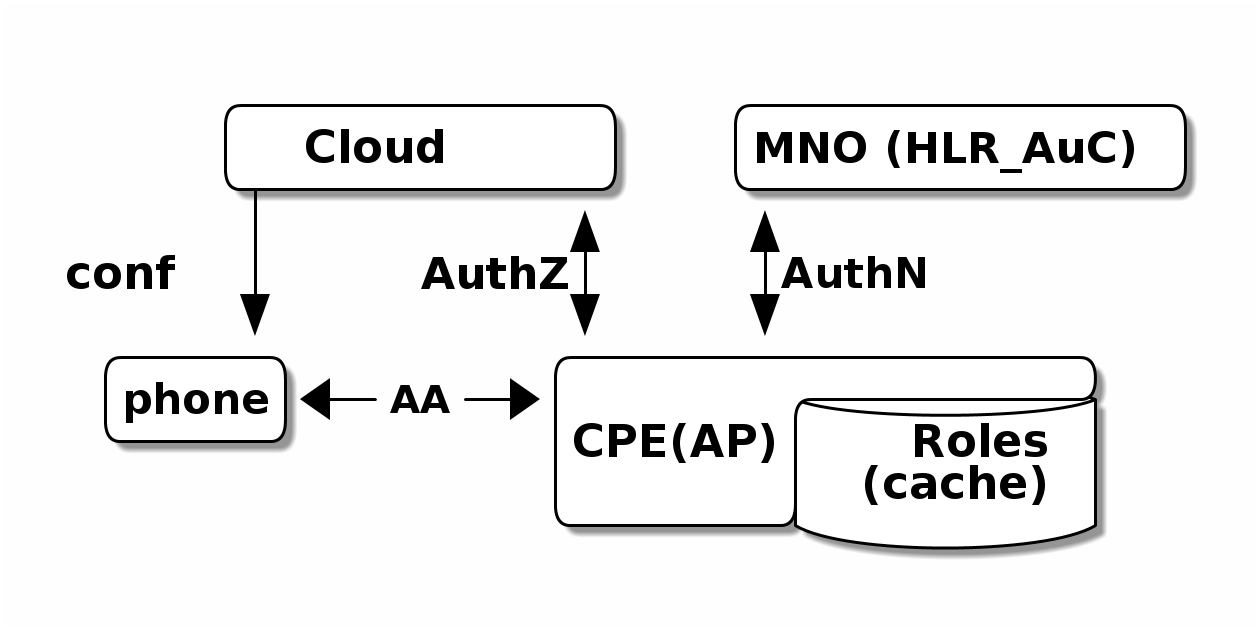
\includegraphics[width=.9\linewidth]{scenVI.png}
\caption{\label{fig:scenario-IV}In the future, CPE could be attached direct to the Cloud and AuthN comes from MNO}
\end{figure}


\section{Bootstrapping with and without PKI}
\label{sec-6-7}
\label{bootstrapping}

Homenet WG proposes the use of Public Key Infrastructure (PKI) at 
home. The public key cryptography is processor intensive and its
asymmetric keys are usually used just in the beginning of
communication. There they can be used to securely negotiate symmetric
keys which allows faster cryptographic processing.
Rest of this section discusses possible PKI usage.

To use PKI for trust anchoring and AuthN in an empty environment, bootstrapping protocols are
first needed.
The bootstrapping protocols in general are used to
bring the first trust anchor in an environment and later use that anchor to
attach other devices to the same trust circle.  A draft from
Behringer\cite{draft-behringer-bootstrap} proposes, that one device
at home is first chosen as a trust anchor  using its unique properties such as 
device Vendor certificates.

Despite the etymology of name bootstrapping, ``Lift oneself by his own
bootstraps'', bootstrapping usually needs some input from outside.
For that, AuthN of the trust anchor device would happen by checking device's Vendor certificates. This anchored
device later becomes home network's Certificate Authority (CA) service
and the trust anchor, upon which the rest of the home network devices
would apply for certificates from to get under the same trust circle.
Key creation, key exchange and their usage is explained in similar
draft from Pritikin\cite{draft-pritikin-bootstrap}. That explains PKI usage in general
in bootstrapping. 


Behringer continues, that this model could be expanded to a full ticket enabled Kerberos style
AA network, where time-limited tickets (tokens) for both
AuthN and AuthZ exist for different services.
Behringer continues, that   end devices could first try to get AuthN ticket,
which does not include yet the AuthZ.
With that ticket, the device may later apply for AuthZ ticket, which
opens the ports to change management service from CPE.
That is very similar to Kerberos, which is based on
Needham-Schroeder protocol.

In GBA, Trusted Third Party authentication center would be setup with the help of MNO.
One service would then authenticate an entity, here smartphone, and
give it a time-limited ticket as a proof that the entity has been authenticated.
When the entity wants to connect to the service, it asks from the central 
server again for ticket, but this time for the service by presenting
the authentication ticket. In return it receives a service ticket which
it can present to the wanted service, who verifies the access based
on the ticket. 

As can be seen, no public key infrastructure (PKI) is used on this.
If EAP-SIM was applied in such environment, it would be used only
once, namely in the bootstrapping phase to setup the CA trust
anchor. Only after that, can the CA start delivering PKI. Kerberos
needs shared keys, and EAP-SIM helps in providing those.


\subsection{this has been said already TB removed.}
\label{sec-6-7-1}
Using tickets has a connection to earlier homenet studies, such as
Behringers work-in-progress
bootstrapping\cite{draft-behringer-bootstrap}.  

 Another bootstrapping architecture is
defined in GBA (General Bootstrapping Architecture), which 
benefits from MNO's or any other identity centre's  knowledge of user's SIM.


In our work, the Authentication server can be an external
RADIUS server, but usually the final decision point lies at the
Authenticator in CPE. Further, in last two planned ways only the
initial bootstrap as well as the change of admin roles and some dangerous
combination of commands would need AA with the smartphone.
Finally this thesis takes the bootstrapped environment as given, i.e.,
the initial configuration has already been set.


\chapter{Conclusion}
\label{sec-7}



The environment described in thesis is a modern complex home network
management, whose configuration management tools are external in the
cloud.  The thesis concentrates on three main parts:
the smartphone driven authorization and authentication at the home
networks, the connection to the existing change management model from
the external cloud service, and the security issues in that environment.

The trust issues between the home network and the cloud are searched
through a smartphone located in the intersection of both domains.
Home Network's future needs, for example the change of the authority
and the delegation of the configuration management have been
described.
To solve those needs, a method to approve changes indirectly has been
proposed. The approval follows from a successful authentication and
authorization with EAP-SIM method by the smartphone and that also sets
a trust anchor to the smartphone.


For testing purposes, a real working EAP-SIM test bed with fake credentials and
a fake mobile operator representing EAP-SIM authentication flow was
built. A dual-role model, which binds the smartphone to the home network and
grants it rights to make changes there, has been proposed.  
An indirect way to approve changes is achieved by binding the authorized
access to the management network. After the authorization, the smart
phone is free to configure the devices with its local application.
Another way to convince the
devices about trusted source is to send approval tickets that can
be verified on reception, but that would involve a more complex setup.

Complexity of existing models in interworking was one motivator for
the work. The research  on the subject did reveal some reasons 
for the complexity, that are difficult to overcome with simplistic 
methods without losing security at the same time.

There are some obvious weaknesses in the proposed solution such as 
missing continuous authorization after management access has been
granted. The application for the smartphone is yet to be implemented.
Possible usage must carefully check the safety limits even when for
example RADIUS protocol still
has strengths in security today. The thesis only scratches bootstrapping
problems and the issues in the home network bootstrapping need to be studied
more thoroughly. A one promising lead would be to use tickets in Kerberized way as in GBA.


After those shortcoming, the provisioning of manager users at home
networks still would minimize with the proposed technique, as the users
already own a smartphone, which is an identifiable and trusted object. As a
positive side effect, the two-factor AuthN from a hardware based SIM would
strengthen an existing security.  Finally, the cloud management tools
would benefit from the trust anchor on the smartphone and could be developed
further to aid in resolving issues in future home networks.

\newpage
%%%%%%%%%%%%%%%
%% BIB
%%%%%%%%%%%%%%%
\bibliographystyle{IEEEtranS}   % already on org header 

\renewcommand{\bibname}{Bibliography}     % Otherwise bilingual babel uses Finnish ``Kirjallisutta''. Strange...
\bibliography{refs}    % already on org header

\addcontentsline{toc}{chapter}{\bibname}  % Include this in TOC

\markboth{\bibname}{\bibname} % Set page header

% not needed \printbibliography                  
% a) heading in English

%%%%%%%%%%%%%
%% APPENDIX
%%%%%%%%%%%%
% if needed, appendix
\appendix
\pagestyle{headings}
%
% a) Not-so-handy way, but at least it works
% 
\def\appA{APPENDIX A. Scripts, confs, and logs} % Define the name and numbering manually
\chapter*{\appA}                       % Create chapter heading
\setcounter{chapter}{1} % Start numbering from zero because command

\markboth{\appA}{\appA}                % Set page header
\addcontentsline{toc}{chapter}{\appA}  % Include this in TOC
% Note that \label does not work with unnumbered chapter

[Appendices are purely optional.  All appendices must be referred to in
the body text, remember this! ]

%\thispagestyle{empty}
\section{shell, logging options}
\label{sec-7-1}
\label{app:fulleap}
\lstset{basicstyle=\ttfamily,columns=fixed}
# % \lstinputlisting[language=bash]
\scriptsize
\lstinputlisting[language=bash]{./testit/apd-tty.clean}
\normalsize



\section{wpa-supplicant settings (wpa-simtest-owrt2.conf)}
\label{sec-7-2}
\label{app:wpa-conf}
\scriptsize
\lstinputlisting[language=sh]{testit/wpa-simtest-owrt2.conf.clean}
\normalsize

\section{RADIUS server conf}
\label{sec-7-3}
\label{app:radius-conf}
\scriptsize
\lstinputlisting[language=sh]{testit/hostapd-jmdemo.conf.clean}
\normalsize
\section{hlr\_auc}
\label{sec-7-4}

\label{app:hlraucgw}
\scriptsize
\lstinputlisting[language=sh]{testit/hostapd-jmdemo.conf.clean}
\normalsize

\scriptsize

\section{No sim}
\label{sec-7-5}
\label{app:nosim}

Here capture + analysis from nosim


\end{otherlanguage} % End on 2nd language part (figures)

\chapter{[MISC to be added on right places]}
\label{sec-8}
\section{facts TBD.}
\label{sec-8-1}
\begin{itemize}
\item ``most EAP authentication protocols lack two features: identity
protection and withstanding man- in-the-middle attacks. ''
\end{itemize}
source :

Yuh-Min Tseng Department of Mathematics, National Changhua University of Education,
Jin-De Campus, Chag-Hua City 500, Taiwan, ROC.

``USIM-based EAP-TLS authentication protocol for
wireless local area networks''
and 

Wireless (In)Security www-page, where 
EAP table shows that PEAP has MiTM.
\url{http://networking.ringofsaturn.com/Security/WirelessInSecurity.php}

\begin{itemize}
\item re-auth for long-lived sessions or if there is cost for disrupting them
\item APs provide different authentication suites for different
\end{itemize}
SSIDs 

\scriptsize
\begin{verbatim}
essid="nurkka"
          IE: IEEE 802.11i/WPA2 Version 1
                        Group Cipher : CCMP
                        Pairwise Ciphers (1) : CCMP
                        Authentication Suites (1) : PSK
essid="simtest"
          IE: IEEE 802.11i/WPA2 Version 1
                        Group Cipher : CCMP
                        Pairwise Ciphers (1) : CCMP
                        Authentication Suites (1) : 802.1x
\end{verbatim}
\normalsize

\section{using EAP for other than network access, i.e., for application auth.}
\label{sec-8-2}
\begin{itemize}
\item \url{http://www.rfc-editor.org/rfc/rfc7057.txt}
\begin{itemize}
\item EAP
\end{itemize}
\item application as an EAP peer
\item RFC6677: Channel-Binding Support for Extensible Authentication Protocol (EAP)
\item channel binding must be used
\end{itemize}

\section{SS7 flaws}
\label{sec-8-3}
German researchers discover a flaw that could let anyone listen to
your cell calls 
Washigtonpost.com 2014/12/18
\section{eap-psk rfc4764.txt}
\label{sec-8-4}
\begin{itemize}
\item other limitations than identity protection are password support and Perfect Forward Secrecy (PFS).
\item eap-psk
\item only 3 standards track EAP methods per IETF terminology,
\end{itemize}
but all of them are deprecated (md5,OTP,GTC ja?)
\begin{itemize}
\item some EAP- o  Essentially require additional infrastructure, e.g., EAP-SIM \footnote{DEFINITION NOT FOUND.},
EAP-AKA \footnote{DEFINITION NOT FOUND.}, or OTP/token card methods like \footnote{DEFINITION NOT FOUND.}.
\end{itemize}


\section{eap-sim acts similar than any other EAP challenge method (or not?)}
\label{sec-8-5}
\begin{itemize}
\item compare eap-sim with other method and point out differences.
\item privacy already shown
\item user defined passwd?
\item how many messages needed? In eap-sim 6+1 (success/failure)
\item to do comparison, I have to study how EAP in general works
\item Authenticator for example can use either local method or
pass-through the authentication to external backend, still keeping
EAP-message in tact(sp?) as of  rfc4137
\item WPA2 package's hostapd from JM does not perhaps provide EAP-PEAPv0 SIM but
\end{itemize}
wpa-supplicant supports.
\begin{itemize}
\item VLAN itself has an attack vector and some methods exists, but also
mitigation for them.
\item rad Authenticator, TLS, RADSEC etc, needs both client\&server in
x509 certificate
\end{itemize}
% Emacs 24.4.1 (Org mode 8.2.10)
\end{document}